\documentclass[]{usiinfprospectus}

\captionsetup{labelfont={bf}}

\author{\centerline{Bevilacqua Joey} \\[3pt] \centerline{De Vita Gianmarco}  \\[3pt] \centerline{Luini Alessandro}  \\[3pt] \centerline{Maggioni Claudio}}

\title{\centerline{Sudoku}}
\versiondate{\today}
\usepackage{boldline} 
\usepackage{enumitem}
\usepackage{listings}
\usepackage[ruled]{algorithm}
\usepackage[noend]{algpseudocode}


\lstdefinestyle{bpstyle}{
  literate={*}{*}1
}

\lstset{
  style=bpstyle
}


\abstract {
The aim of this project is to make an Encoder and Decoder for a SAT-solver in order to decide whether a problem is satisfiable or unsatisfiable. WRITE A BETTER ABSTRACT
}

% For Sudoku drawing
\usepackage{tikz}
\newcounter{row}
\newcounter{col}

\newcommand\setrow[9]{
  \setcounter{col}{1}
  \foreach \n in {#1, #2, #3, #4, #5, #6, #7, #8, #9} {
    \edef\x{\value{col} - 0.5}
    \edef\y{9.5 - \value{row}}
    \node[anchor=center] at (\x, \y) {\n};
    \stepcounter{col}
  }
  \stepcounter{row}
}

\begin{document}
\maketitle
\tableofcontents
\newpage
%%%%%%%%%%%%%%%%%%%%%%%%%
\section{Introduction} \label{introduction}
Even though Sudoku is a Japanese word, literally meaning "single digit", according to some sources it was actually invented in Switzerland by the already famous mathematician Euler from Basel. However, it is generally acknowledged that the origin of this game is European (around XIX century) and that the modern and common version has been realized in the United States in the second half of the XX century named as "Number Place", from which it spread across the globe, even in Japan, where it took the famous name it is known with.\\ \\
The aim of this homework is to make an Encoder and Decoder for a SAT-solver in order to decide whether a problem is satisfiable or unsatisfiable. 
\newpage
\section{Problem definition} \label{problem}
Sudokus are puzzles based upon number placement. They are classically structured in a $9\times 9$ grid with 81 cells, divided into $3\times 3$ boxes. In order to be satisfiable, the following statements must hold:
\begin{itemize}%[label={(\arabic*)}]
\item In every cell there is exactly one number $c \in \{1, 2, ..., 9 \}$
\item No number may appear more than once in the same row.
\item No number may appear more than once in the same column.
\item No number may appear more than once in the same box.
\end{itemize}
Often Sudoku puzzles are initialized with some values placed, leaving blank spaces to be filled by the player with values respecting the rules above. Visually, Sudokus appear as a square grid, an example can be the following:

%Draw Sudoku
\begin{figure}[h]
\begin{center}
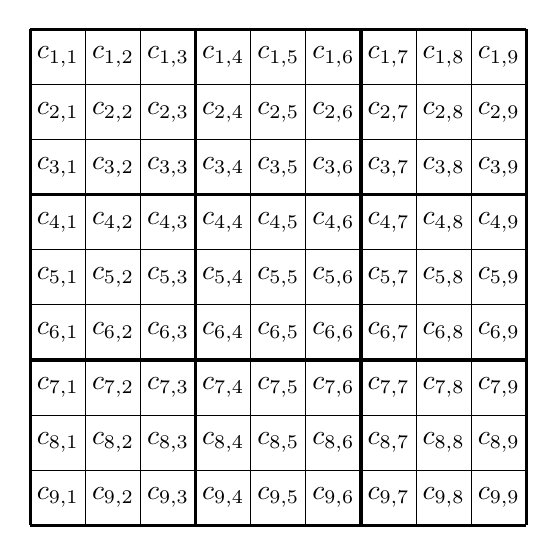
\begin{tikzpicture}[scale=.7]
  \begin{scope}
    \draw (0, 0) grid (9, 9);
    \draw[very thick, scale=3] (0, 0) grid (3, 3);

    \setcounter{row}{1}
    \foreach \i in {1,...,9}
    {
    \setrow {$c_{\i,1}$ }{$c_{\i,2}$}{$c_{\i,3}$}  {$c_{\i,4}$}{$c_{\i,5}$}{$c_{\i,6}$}  {$c_{\i,7}$}{$c_{\i,8}$}{$c_{\i,9}$}
    }
  \end{scope}
\end{tikzpicture}
\end{center}
\caption{A $9\times 9$ Sudoku puzzle.}
\end{figure}
\noindent
Assuming that every $c_{i,j}$ in the Sudoku grid in Figure 1 takes just a value in interval \{1,2,...,9\}, such solution can be considered valid if and only if the following conditions are satisfied: 
\begin{enumerate}[label={(\arabic*)}]
\item In every row $i$ (i.e., $c_{i,1}$, $c_{i,2}$, ..., $c_{i,9}$) there is at least one element that takes one value in \{1,2,...,9\}, but all values from 1 to 9 must be taken. Since in a row there are only 9 elements, it means that there will be a one-to-one mapping from these row elements to the \{1,2,...,9\} set values, thus each row will be made of nine different numbers.
\item In every column $j$ (i.e., $c_{1,j}$, $c_{2,j}$, ..., $c_{9,j}$) there is at least one element that takes one value in \{1,2,...,9\}, but all values from 1 to 9 must be taken. Since in a column there are only 9 elements, it means that there will be a one-to-one mapping from these column elements to the \{1,2,...,9\} set values, thus each column will be made of nine different numbers.
\item In every box, no number may appear more than once. Since a box is made up by 9 elements, it means that each box will contain all the values within the \{1,2,...,9\} set. What requires a bit more of reasoning here is finding a generalizing way to define all the elements in a box for every box. While for rows and columns it suffices to use a matrix-like notation, here some background reasoning is needed. It can be noticed that, in every box, the following pattern can be observed:
\begin{figure}[h]
\begin{center}
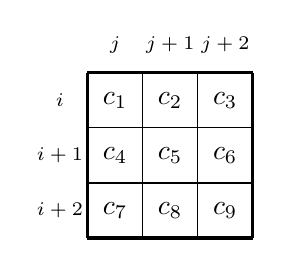
\begin{tikzpicture}[scale=.7]
  	\begin{scope}
    	\draw (0, 0) grid (3, 3);
   	\draw[very thick, scale=3] (0, 0) grid (1, 1);
   	
   	\node[anchor=center] at (0.5, 3.5) {\scriptsize{$j$}};
   	\node[anchor=center] at (1.5, 3.5) {\scriptsize{$j+1$}};
   	\node[anchor=center] at (2.5, 3.5) {\scriptsize{$j+2$}};
   	
   	\node[anchor=center] at (-0.5, 2.5) {\scriptsize{$i$}};
   	\node[anchor=center] at (-0.5, 1.5) {\scriptsize{$i+1$}};
   	\node[anchor=center] at (-0.5, 0.5) {\scriptsize{$i+2$}};

   	\node[anchor=center] at (0.5, 2.5) {$c_1$};
   	\node[anchor=center] at (1.5, 2.5) {$c_2$};
   	\node[anchor=center] at (2.5, 2.5) {$c_3$};
   	
   	\node[anchor=center] at (0.5, 1.5) {$c_4$};
   	\node[anchor=center] at (1.5, 1.5) {$c_5$};
   	\node[anchor=center] at (2.5, 1.5) {$c_6$};

   	\node[anchor=center] at (0.5, 0.5) {$c_7$};
   	\node[anchor=center] at (1.5, 0.5) {$c_8$};
   	\node[anchor=center] at (2.5, 0.5) {$c_9$};
   	
  	\end{scope}
\end{tikzpicture}
\end{center}
\caption{A $3\times 3$ Sudoku generalized box.}
\end{figure}

\noindent
That means that every box has its top-leftmost cell at a particular coordinate ($i,\,j$) and its other corner cells are clockwise respectively at coordinates: ($i,\,j+2$),  ($i+2,\,j+2$) and ($i+2,\,j$). By this, it can be said that by individuating the top-leftmost cell of a box it is possible to individuate the box itself. Hence, for $i=1$ and $j=1$, we have corner cells ($1,\,1$), ($1,\,3$),  ($3,\,3$) and ($3,\,1$), that is the top-leftmost box in the Sudoku grid. From this approach, the boxes making up the grid can be defined as:
\begin{figure}[h]
\begin{center}
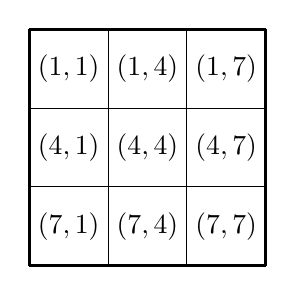
\begin{tikzpicture}[scale=1]
  	\begin{scope}
    	\draw (0, 0) grid (3, 3);
   	\draw[very thick, scale=3] (0, 0) grid (1, 1);
   	
   	\node[anchor=center] at (0.5, 2.5) {$(1,1)$};
   	\node[anchor=center] at (1.5, 2.5) {$(1,4)$};
   	\node[anchor=center] at (2.5, 2.5) {$(1,7)$};
   	
   	\node[anchor=center] at (0.5, 1.5) {$(4,1)$};
   	\node[anchor=center] at (1.5, 1.5) {$(4,4)$};
   	\node[anchor=center] at (2.5, 1.5) {$(4,7)$};

   	\node[anchor=center] at (0.5, 0.5) {$(7,1)$};
   	\node[anchor=center] at (1.5, 0.5) {$(7,4)$};
   	\node[anchor=center] at (2.5, 0.5) {$(7,7)$};
   	
  	\end{scope}
\end{tikzpicture}
\end{center}
\caption{A $9\times 9$ Sudoku grid. Each square corresponds to a $3\times 3$ box. Inside of the square, the ($i,\,j$) coordinate of the top-leftmost cell of that box is written.}
\end{figure}

\noindent
It can be seen that the coordinates are nothing but all the possible permutations of three values: 1, 4 and 7. From this, we can define a set $B=\{1,\,4,\,7\}$ containing these values.\\
\end{enumerate}
\newpage
\section{Encoder and Decoder}\label{encdec}
\noindent
Let \textbf{is\_valid} define whether a row, column or box is valid. That means that the nine elements along a row, column or within a box must be different and equal to a digit in set $\{1,2,...,9\}$, thus meaning that a row, column or box is valid if it contains all digits. Let's consider $c_1,\,c_2,\,...,\,c_9$, which may be the elements within a row, column or box. Then we have:
\begin{align*}
\text{is\_valid}\left(  c_1,  c_2,  c_3,  c_4,  c_5,  c_6,  c_7,  c_8,  c_9  \right) = & \\
& \left(  c_1 \vee  c_2 \vee c_3 \vee c_4 \vee  c_5 \vee  c_6 \vee  c_7 \vee  c_8 \vee  c_9  \right)\\
& \wedge \left(  c_1 \vee  c_2 \vee c_3 \vee c_4 \vee  c_5 \vee  c_6 \vee  c_7 \vee  c_8 \vee  c_9  \right)\\
& \wedge \left(  c_1 \vee  c_2 \vee c_3 \vee c_4 \vee  c_5 \vee  c_6 \vee  c_7 \vee  c_8 \vee  c_9  \right)\\
& \wedge \left(  c_1 \vee  c_2 \vee c_3 \vee c_4 \vee  c_5 \vee  c_6 \vee  c_7 \vee  c_8 \vee  c_9  \right)\\
& \wedge \left(  c_1 \vee  c_2 \vee c_3 \vee c_4 \vee  c_5 \vee  c_6 \vee  c_7 \vee  c_8 \vee  c_9  \right)\\
& \wedge \left(  c_1 \vee  c_2 \vee c_3 \vee c_4 \vee  c_5 \vee  c_6 \vee  c_7 \vee  c_8 \vee  c_9  \right)\\
& \wedge \left(  c_1 \vee  c_2 \vee c_3 \vee c_4 \vee  c_5 \vee  c_6 \vee  c_7 \vee  c_8 \vee  c_9  \right)\\
& \wedge \left(  c_1 \vee  c_2 \vee c_3 \vee c_4 \vee  c_5 \vee  c_6 \vee  c_7 \vee  c_8 \vee  c_9  \right)\\
& \wedge \left(  c_1 \vee  c_2 \vee c_3 \vee c_4 \vee  c_5 \vee  c_6 \vee  c_7 \vee  c_8 \vee  c_9  \right)\\
= & \bigwedge^9_{i=1}  \bigvee^9_{i=1} \,\,\, c_i
\end{align*}

\noindent
Now, since we have given a definition of valid, we can say that a Sudoku is valid if and only if: 
\begin{enumerate}[label={(\arabic*)}]
\item Every row is valid.
\item Every column is valid.
\item Every box is valid.
\end{enumerate}

\noindent
Therefore, the Sudoku problem for a 9x9 grid can be defined as:
\setcounter{equation}{0}
\begin{align}
\text{sudoku}\left( \{ c_{i,j} \}_{i, j \in \{ 1,...,9\}} \right) = & \nonumber\\
&\bigwedge^9_{i=1} \text{ is\_valid}\left(  c_{i,1},  c_{i,2},  c_{i,3},  c_{i,4},  c_{i,5},  c_{i,6},  c_{i,7},  c_{i,8},  c_{i,9}  \right)\\
\wedge &\bigwedge^9_{j=1} \text{ is\_valid}\left( c_{1,j},  c_{2,j},  c_{3,j},  c_{4,j},  c_{5,j},  c_{6,j},  c_{7,j},  c_{8,j},  c_{9,j} \right) \\
\wedge &\bigwedge^9_{i,j \in \{1,\,4,\,7\}} \text{ is\_valid}\left( c_{i,1},  c_{i,(j+1)},  c_{i,3},  c_{i,4},  c_{i,5},  c_{i,6},  c_{i,7},  c_{i,8},  c_{i,9} \right).
\end{align}
\newpage
\section{Development}\label{development}
We have developed the project in Python3 to provide both a web interface and the solver logic using z3.\\
For what concerns the z3 SAT solver, we have used the official \texttt{z3–solver} Python3 library to write the z3 logic instead of writing a z3 \texttt{.dimacs} file for every execution and invoking the z3 solver using a system shell. This allows for better performance and easier maintenance of the code.
The \texttt{z3–solver} Python3 library allows to specify constraints programmatically and is able to provide both information about the satisfiability information and data structure models that represent a valid solution for the problem.\\ \\
First of all, we want to translate the following definition into Python3 \texttt{z3–solver} code:
\begin{align*}
\text{sudoku}\left( \{ c_{i,j} \}_{i, j \in \{ 1,...,9\}} \right) = & \nonumber\\
       & \bigwedge^9_{i=1} \text{ is\_valid}\left(  c_{i,1},  c_{i,2},  c_{i,3},  c_{i,4},  c_{i,5},  c_{i,6},  c_{i,7},  c_{i,8},  c_{i,9}  \right)\\
\wedge &\bigwedge^9_{j=1} \text{ is\_valid}\left( c_{1,j},  c_{2,j},  c_{3,j},  c_{4,j},  c_{5,j},  c_{6,j},  c_{7,j},  c_{8,j},  c_{9,j} \right) \\
\wedge &\bigwedge^9_{i,j \in B} \text{ is\_valid}\left( c_{i,1},  c_{i,(j+1)},  c_{i,3},  c_{i,4},  c_{i,5},  c_{i,6},  c_{i,7},  c_{i,8},  c_{i,9} \right).
\end{align*}

\noindent
Here we build three list of conditions that should all be satisfied: the first condition guarantees that each row does not contain any repeated element within itself. The second condition guarantees that each column does not contain any repeated element while the third one, as described previously
in section~\ref{problem}, guarantees the uniqueness of each element in the 9 boxes of our Sudoku board. Now, it follows the pseudo-code algorithm that we designed and was used as a basis for the \texttt{z3–solver} API in the Python3 implementation.
\begin{algorithm}[H]
\hspace*{\algorithmicindent} \textbf{Input}: $c$, Sudoku board. \\
\hspace*{\algorithmicindent} \textbf{Output}: $s$, solver. 
\begin{algorithmic}[1]\label{algorithm:}
\Function {BuildSolver}{$c$}
\State {\textsc{RowsCheck} $\gets$ []} \Comment{Create array for rows check}
\For {$i$ in range $[1,9]$}\Comment{Go across nine elements}
\State {\textsc{RowsCheck}.\textsc{push}$\left(\textsc{isValid}(c_{1,i},\, c_{2,i},\, c_{3,i},\, c_{4,i},\, c_{5,i},\, c_{6,i},\, c_{7,i},\, c_{8,i},\, c_{9,i}) \right)$}
\EndFor
\State {\textsc{ColumnsCheck} $\gets$ []} \Comment{Create array for columns check}
\For {$i$ in range $[1,9]$}\Comment{Go across nine elements}
\State {\textsc{ColumnsCheck}.\textsc{push}$\left(\textsc{isValid}(c_{i,1},\, c_{i,2},\, c_{i,3},\, c_{i,4},\, c_{i,5},\, c_{i,6},\, c_{i,7},\, c_{i,8},\, c_{i,9}) \right)$}
\EndFor
\State {\textsc{BoxesCheck} $\gets$ []} \Comment{Create array for boxes check}
\For {$i$ in range $[1,9]$ step = 3}
\For {$j$ in range $[1,9]$ step = 3}
\State {\textsc{BoxesCheck}.\textsc{push}$\left(\textsc{isValid}(c_{i,j},\, c_{i,j+1},\, c_{i,j+2},\, c_{1+1,j},\, c_{i+1,j+1},\, c_{i+1,j+2},\, c_{i+2,j},\, c_{i+2,j+1},\, c_{i+2,j+2}) \right)$}
\EndFor
\EndFor
\State{\textsc{s} $\gets$ \textsc{Z3Solver()}}
\State{\textsc{s}.\textsc{add}$\left( \textsc{And} \left( \textsc{And} \left( \textsc{RowsCheck}\right),\, \textsc{And} \left( \textsc{ColumnsCheck}\right),\,\textsc{And} \left( \textsc{BoxesCheck}\right) \right) \right)$}\\
\Return {$s$}
\EndFunction
\end{algorithmic}
\caption {Build Solver Algorithm}
\end{algorithm}

\newpage
\noindent
Now we want to write the $ is\_valid $ formulation as Python3 \texttt{z3–solver}
code:

\begin{align*}
\text{is\_valid}\left(  c_1,  c_2,  c_3,  c_4,  c_5,  c_6,  c_7,  c_8,  c_9  \right) = \bigwedge^9_{i=1}  \bigvee^9_{i=1} \,\,\, c_i
\end{align*}

\begin{algorithm}[H]
\hspace*{\algorithmicindent} \textbf{Input}: $c$, Sudoku board. \\
\hspace*{\algorithmicindent} \textbf{Output}: $s$, solver. 
\begin{algorithmic}[1]\label{algorithm:}
\Function {isValid}{$c$}
\State {\textsc{x} $\gets$ []} \Comment{Create array}
\For {$i$ in range [1,9]}
\If {$c_i$.\textsc{isNumeric()}}
\State{\textsc{x.push}($c_i$)}
\Else
\State{\textsc{x.push}($c_i$)}
\EndIf
\EndFor
\For {$d$ in range [1,9]}
\State {\textsc{orArgs $\gets$ []}}
\For {$d$ in range [1,9]}
\State {\textsc{orArgs.push($x_i == d$)}}
\EndFor
\State {\textsc{andArgs.push(Or(orArgs))}}
\EndFor\\
\Return {$\textsc{And(andArgs)}$}
\EndFunction
\end{algorithmic}
\caption {Build Solver Algorithm}
\end{algorithm}

\newpage
\section{Instructions for running}

In order to run the Sudoku SAT solver, you first need to install Python3 (available at \url{https://www.python.org/downloads/}). Then you need to open the terminal and browse to the project directory using the \texttt{cd}
command. Once you have reached the destination folder which is the project directory, run the following command to install the dependencies using the Python3 \texttt{pip} command (that literally stands for ``pip install package'', according to its \href{https://en.wikipedia.org/wiki/Pip\_(package\_manager)}{Wikipedia page}):

\begin{center}
\texttt{pip install -r requirements.txt}
\end{center}

\noindent
Finally, now that you have installed the dependencies, you can now start the Flask server. Flask is a web server framework for Python3, see the \href{https://flask.palletsprojects.com/}{official documentation}.\\ \\
Run this command to start the Sudoku SAT Solver:

\begin{center}
\texttt{FLASK\_APP=solver/app flask run}
\end{center}

\noindent
And finally open the \url{http://localhost:5000/} website to visit the local
instance of the Sudoku SAT Solver project.


\section{Trials}\label{trials}


\begin{figure}
\caption{The web app UI}
\centering
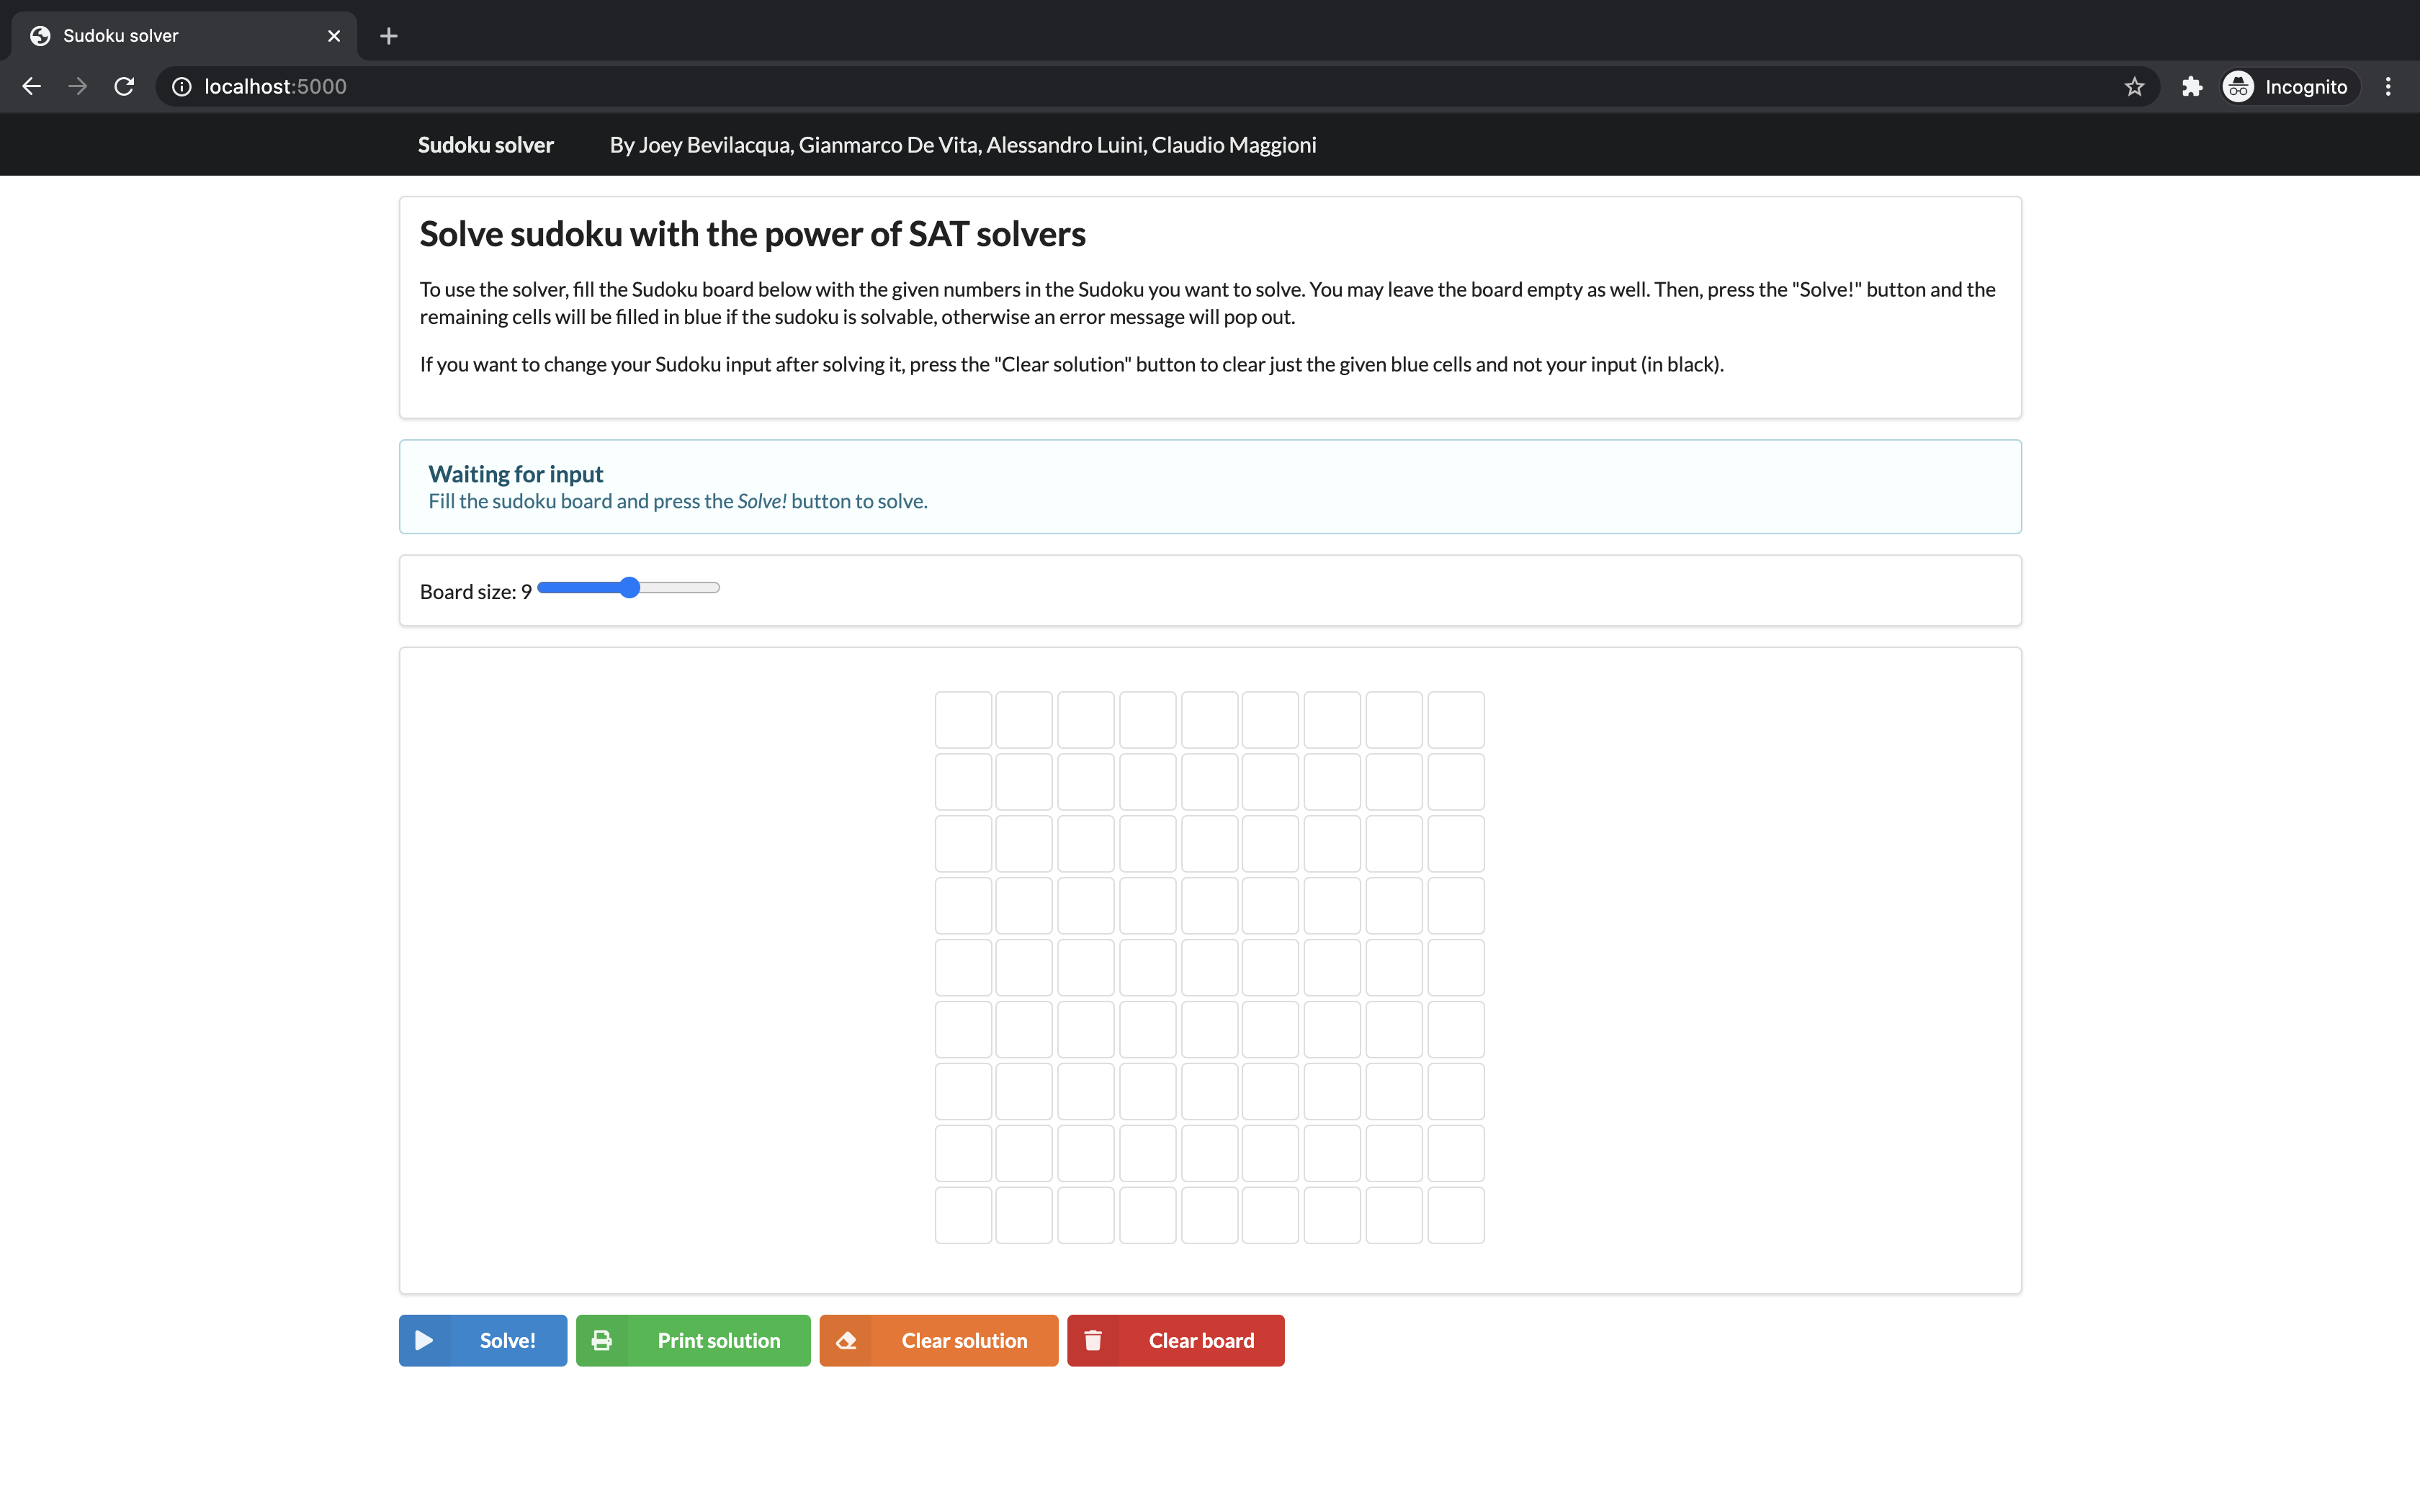
\includegraphics[width=0.8\textwidth]{pics/app_ui.png}
\end{figure}

\begin{figure}
\caption{Fill the sudoku board}
\centering
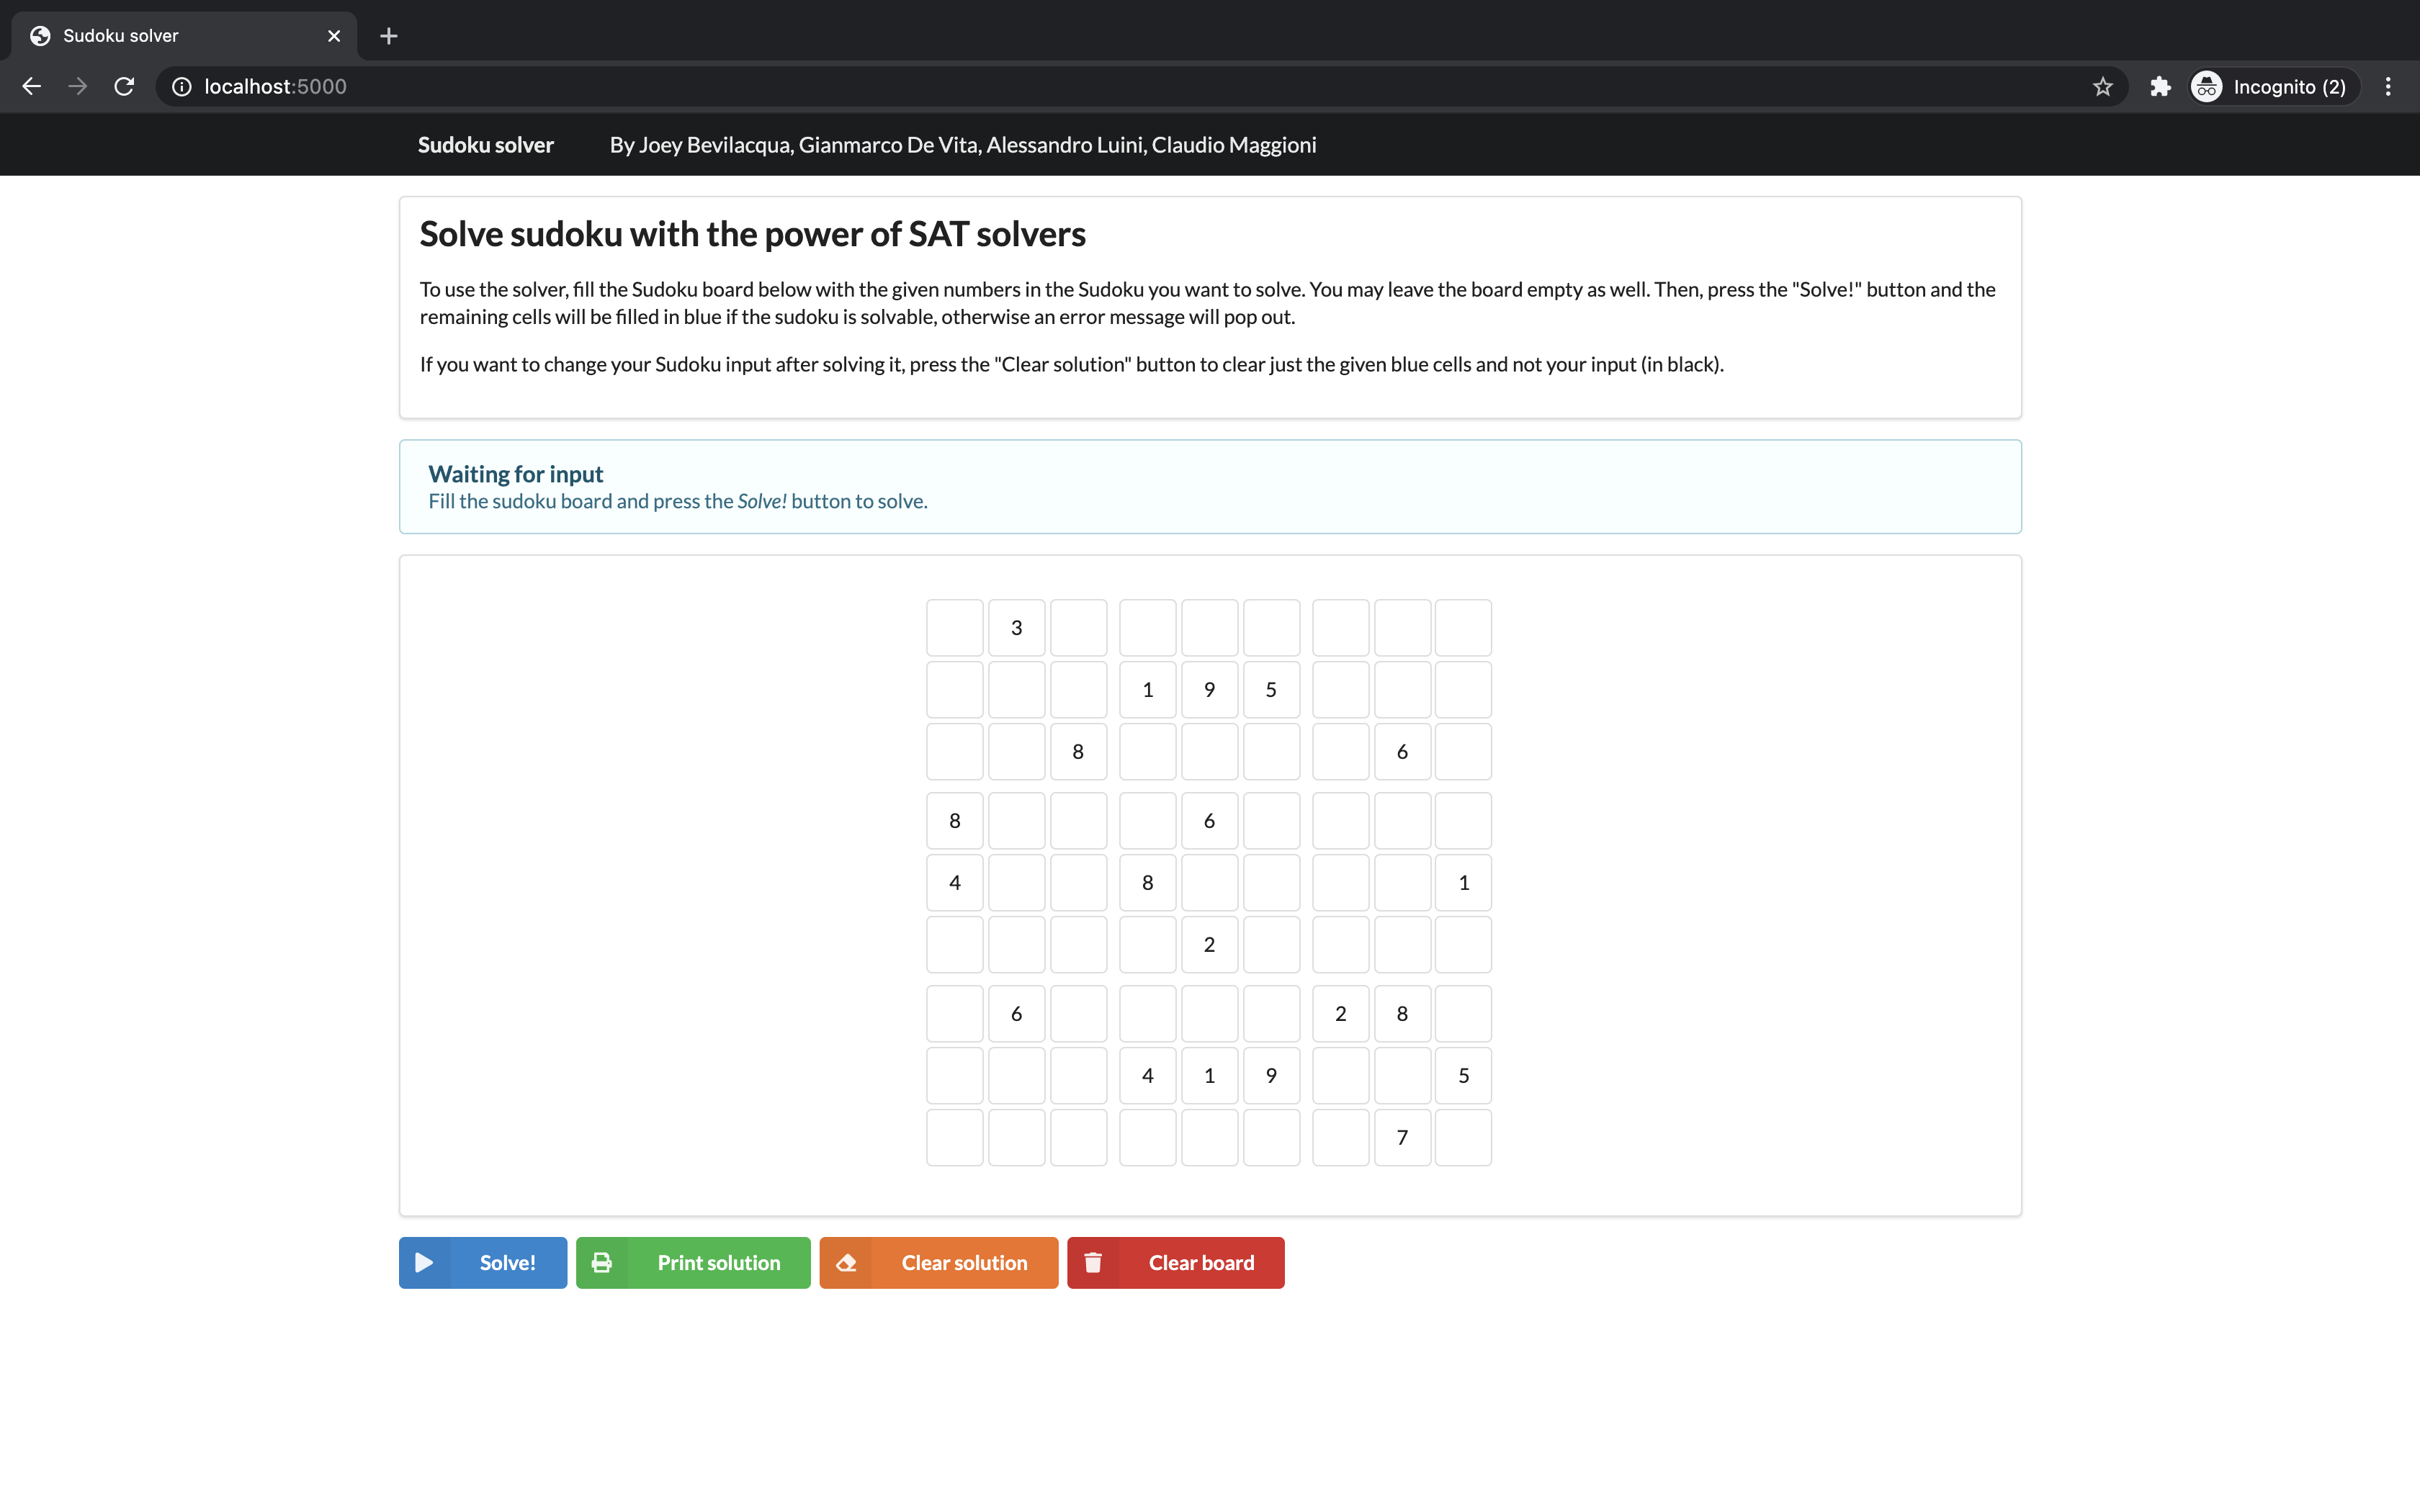
\includegraphics[width=0.8\textwidth]{pics/fill_board.png}
\end{figure}

\begin{figure}
\caption{Press the \texttt{Solve} button to find the soluscion}
\centering
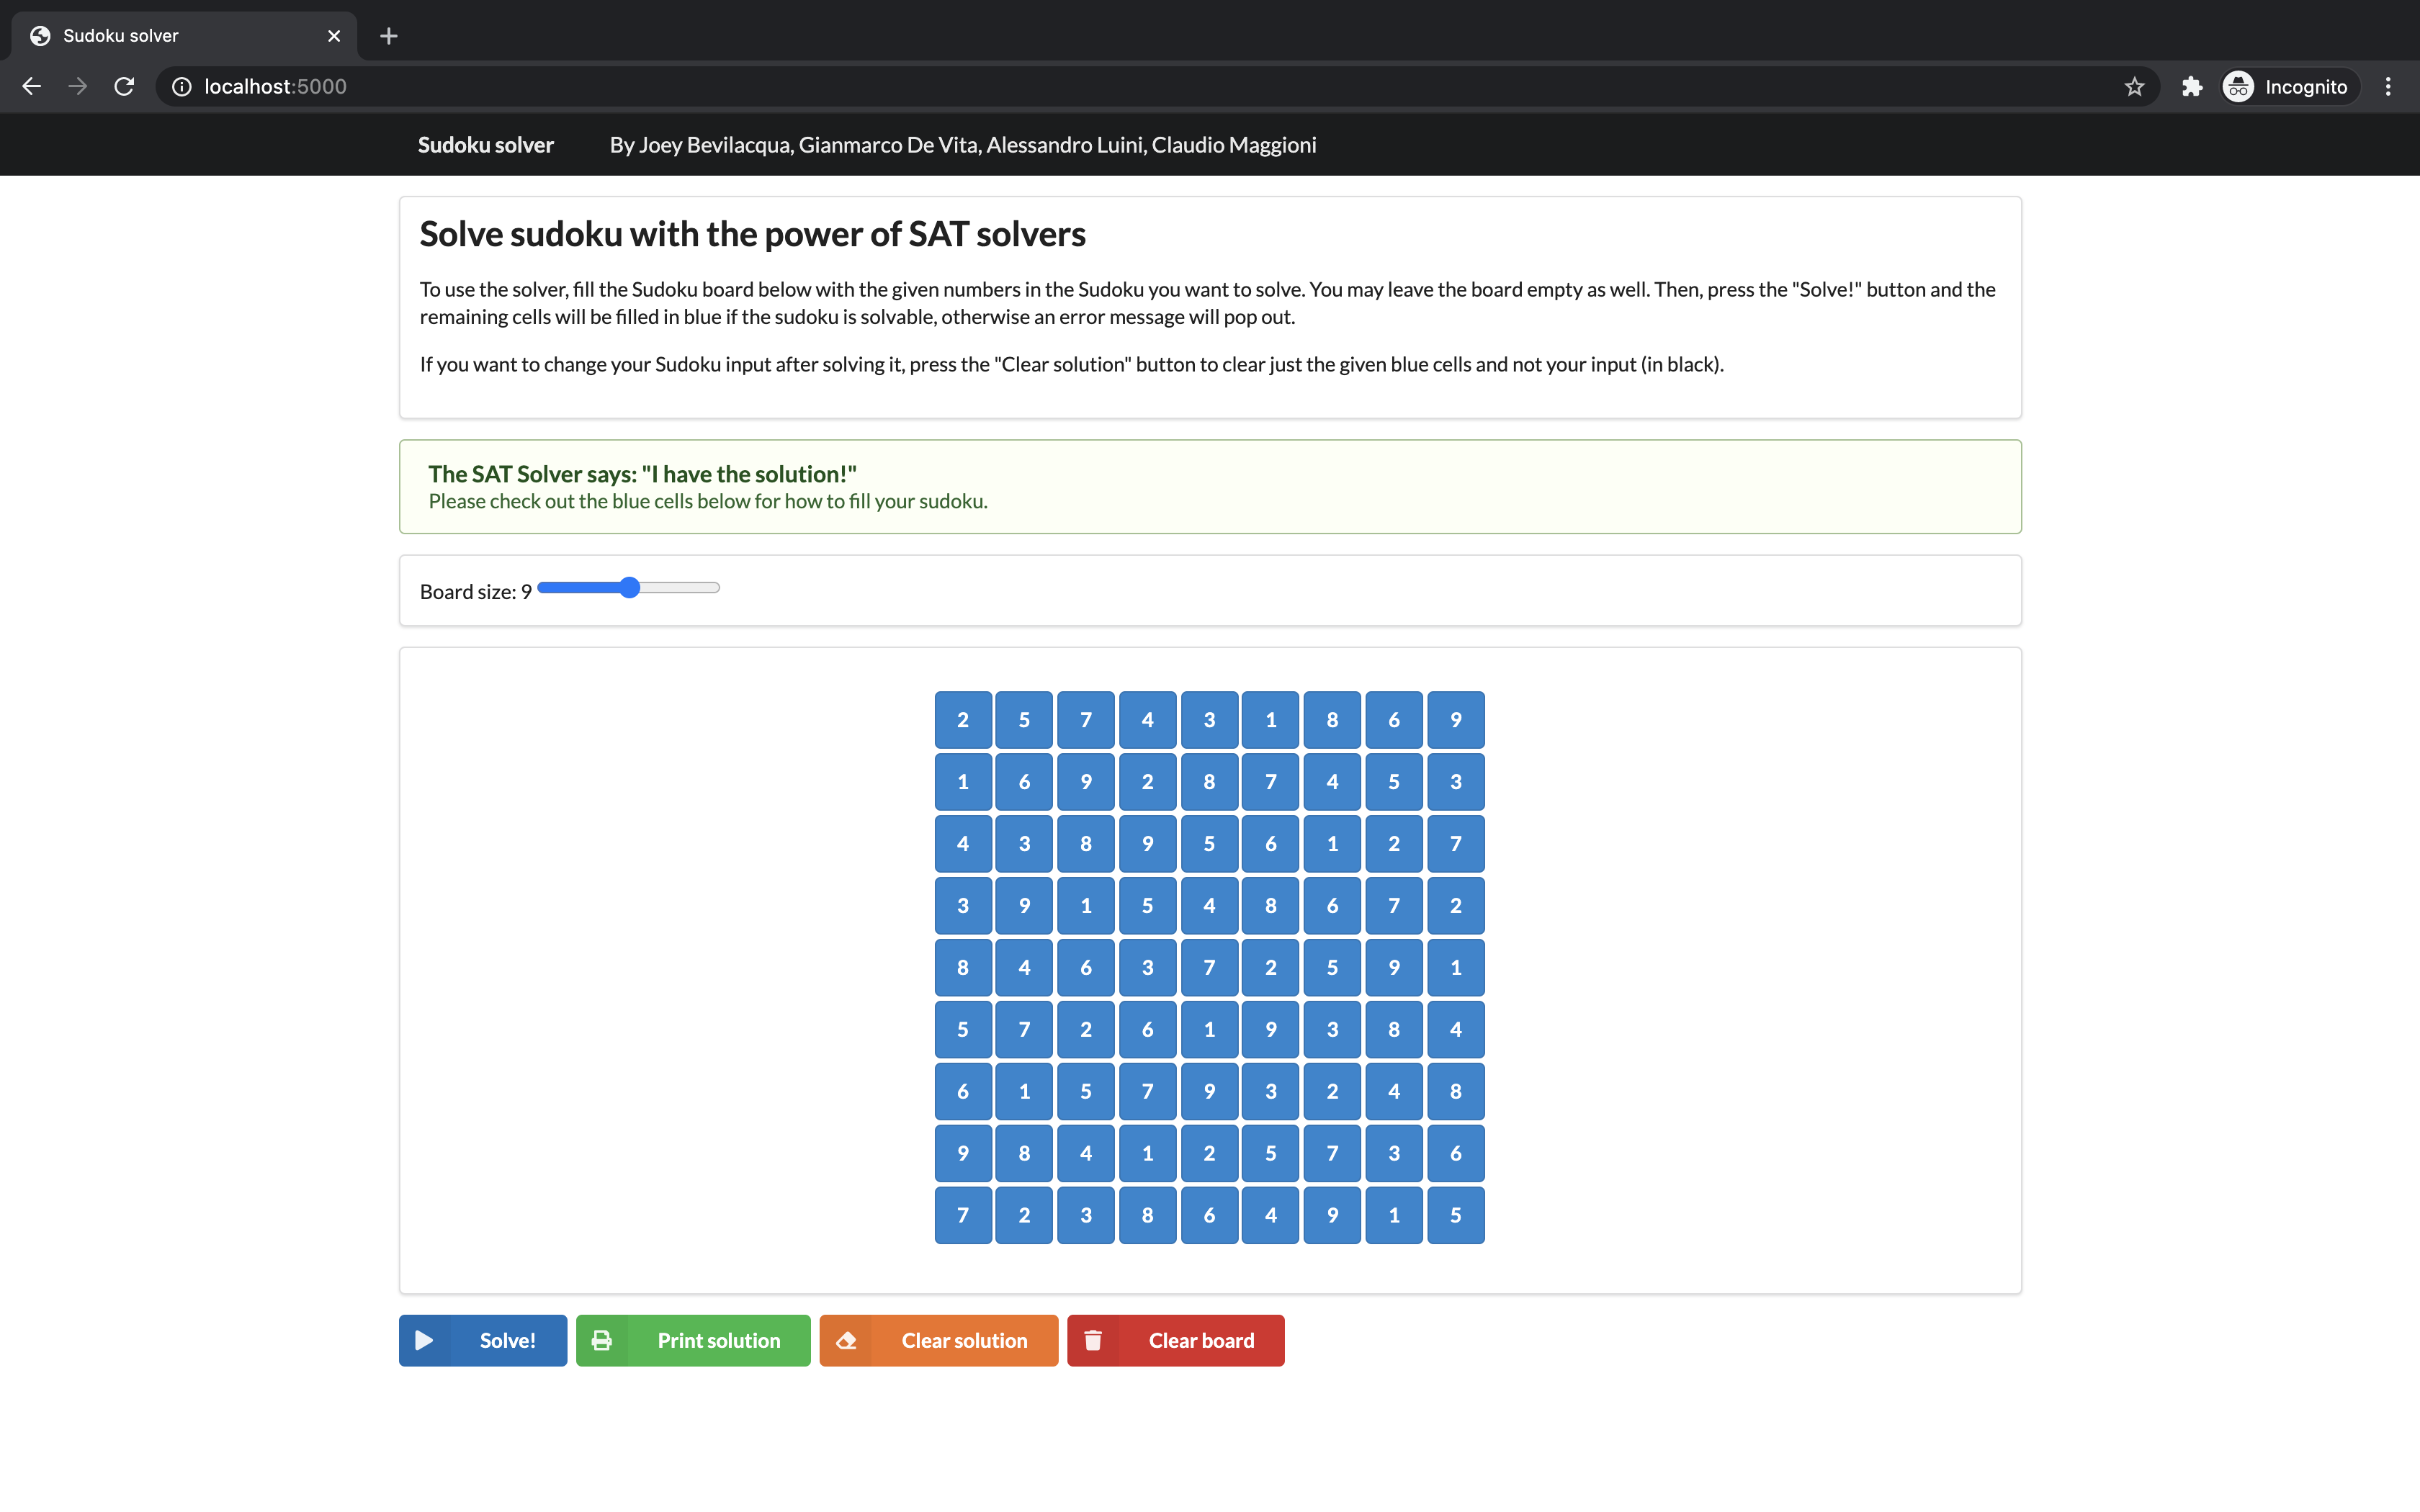
\includegraphics[width=0.8\textwidth]{pics/solved.png}
\end{figure}

\begin{figure}
\caption{Errors if a number appears multiple times in the same row}
\centering
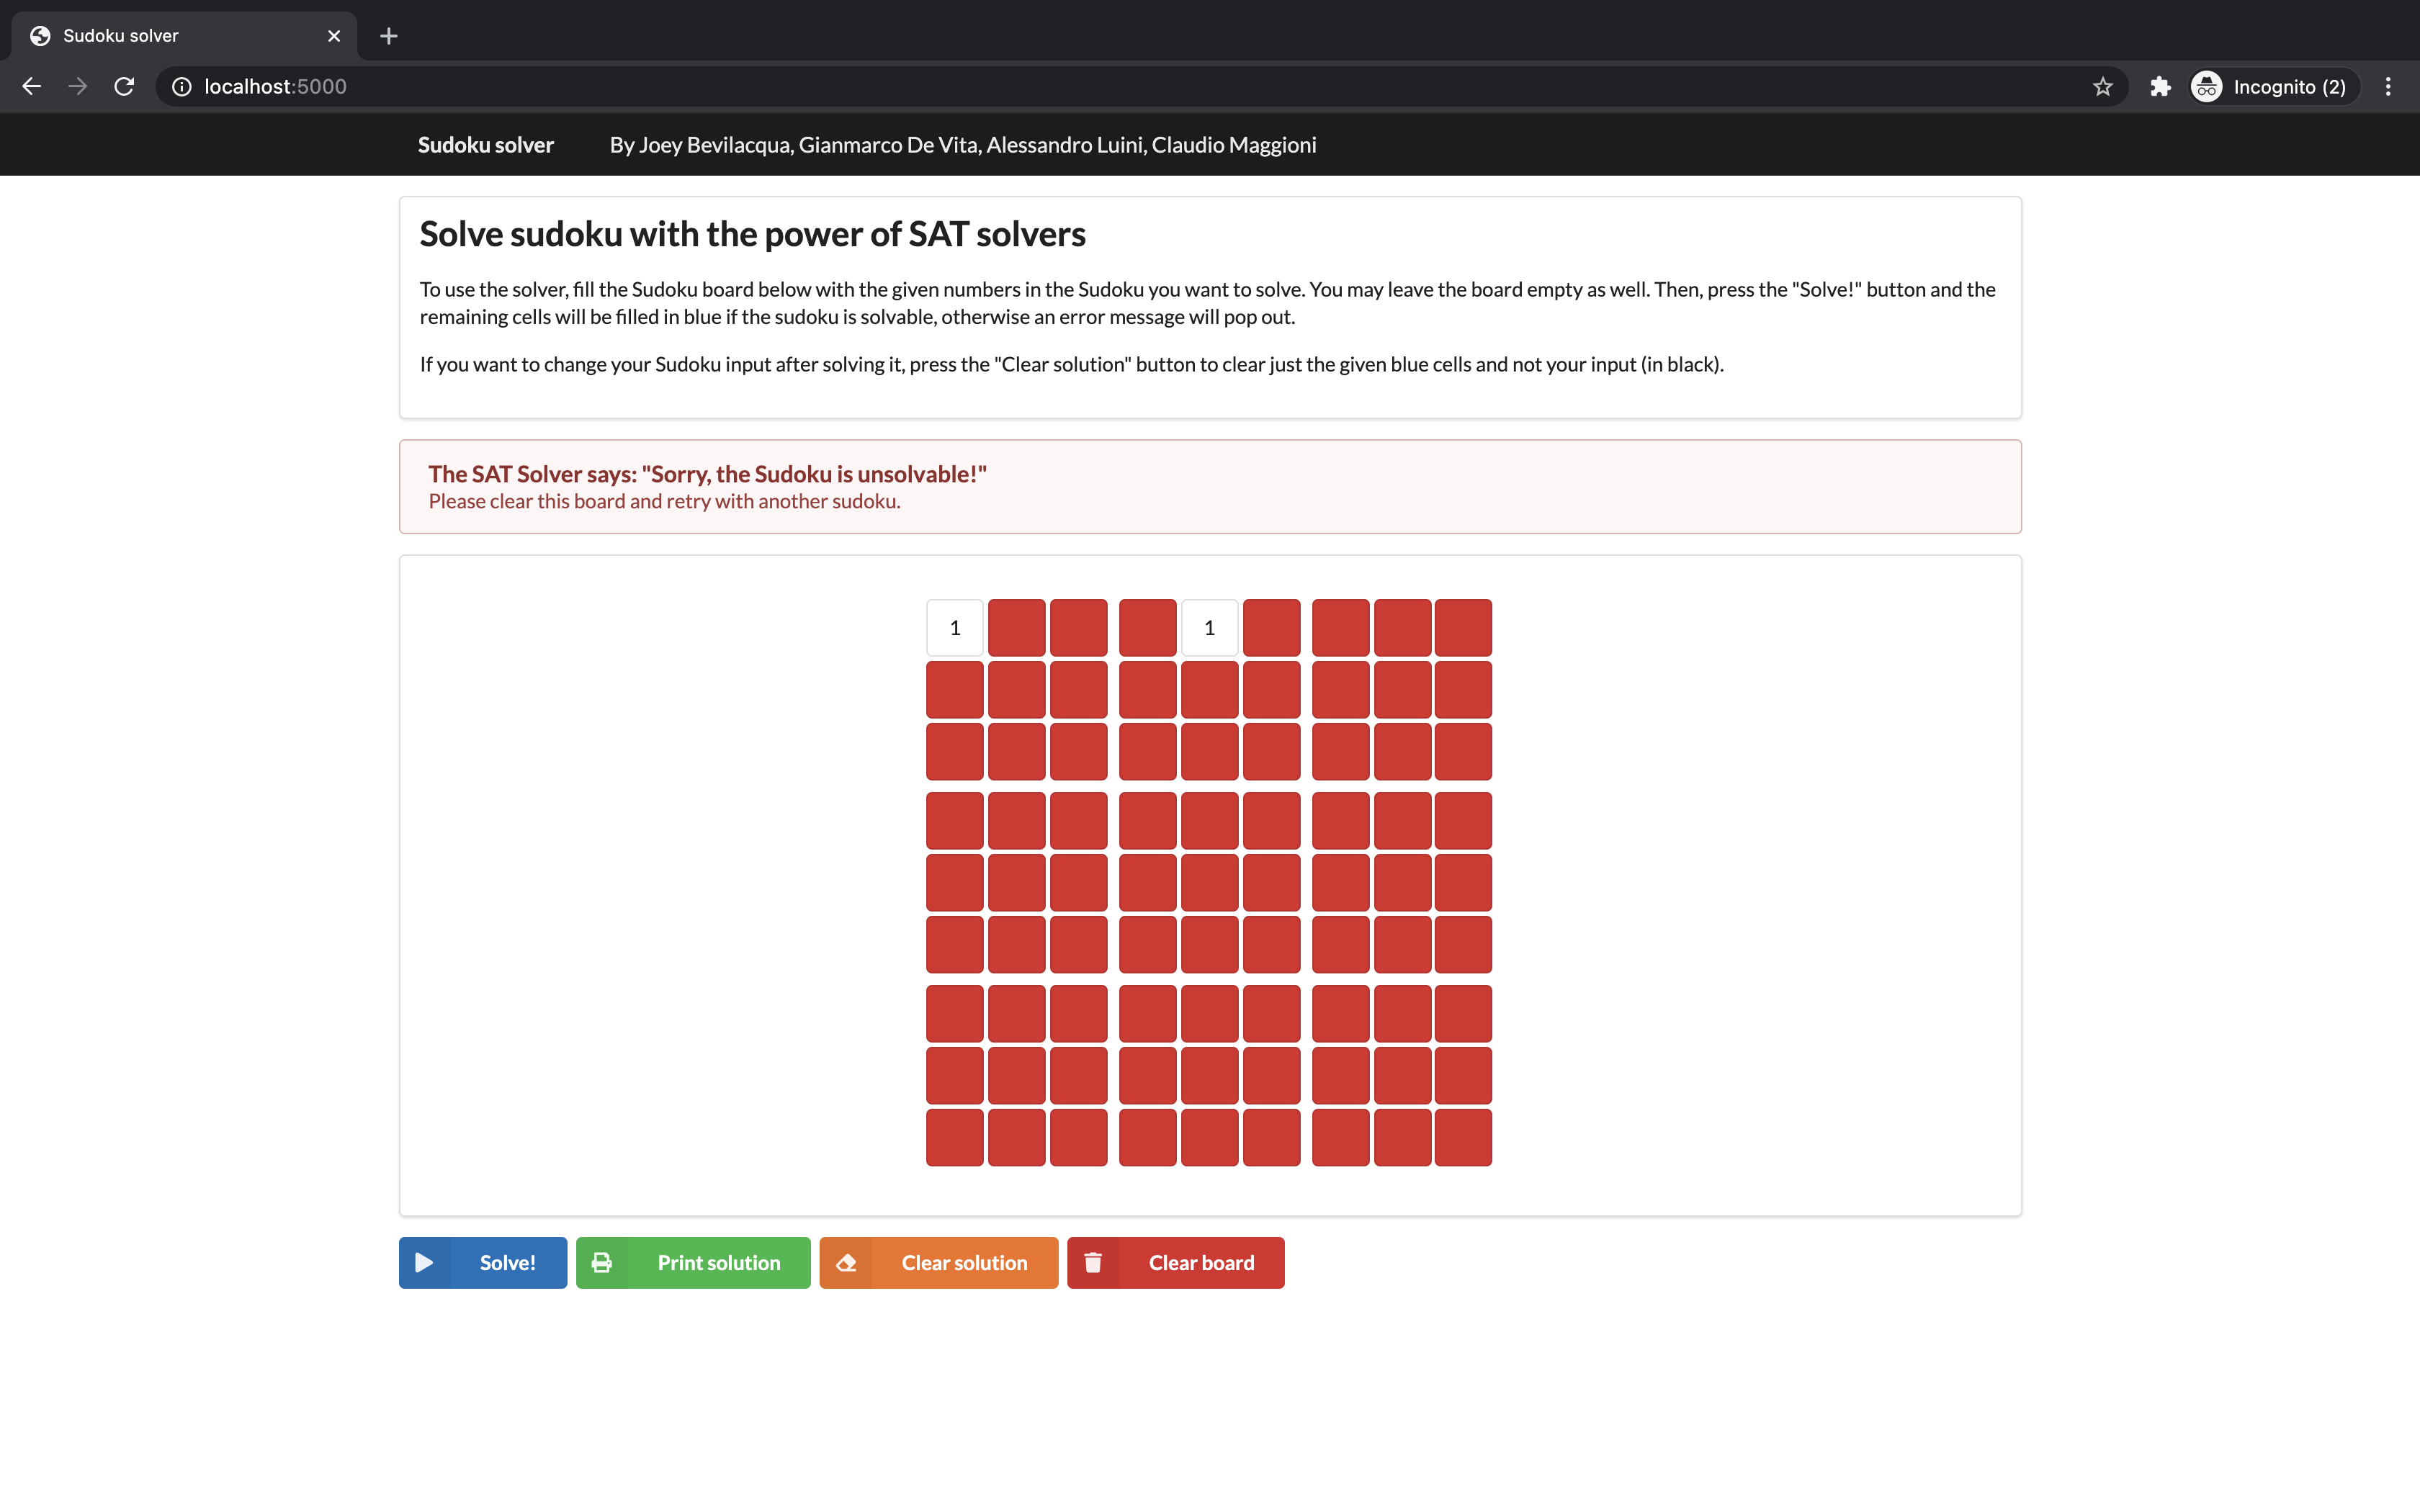
\includegraphics[width=0.8\textwidth]{pics/row_check.png}
\end{figure}

\begin{figure}
\caption{Errors if a number appears multiple times in the same column}
\centering
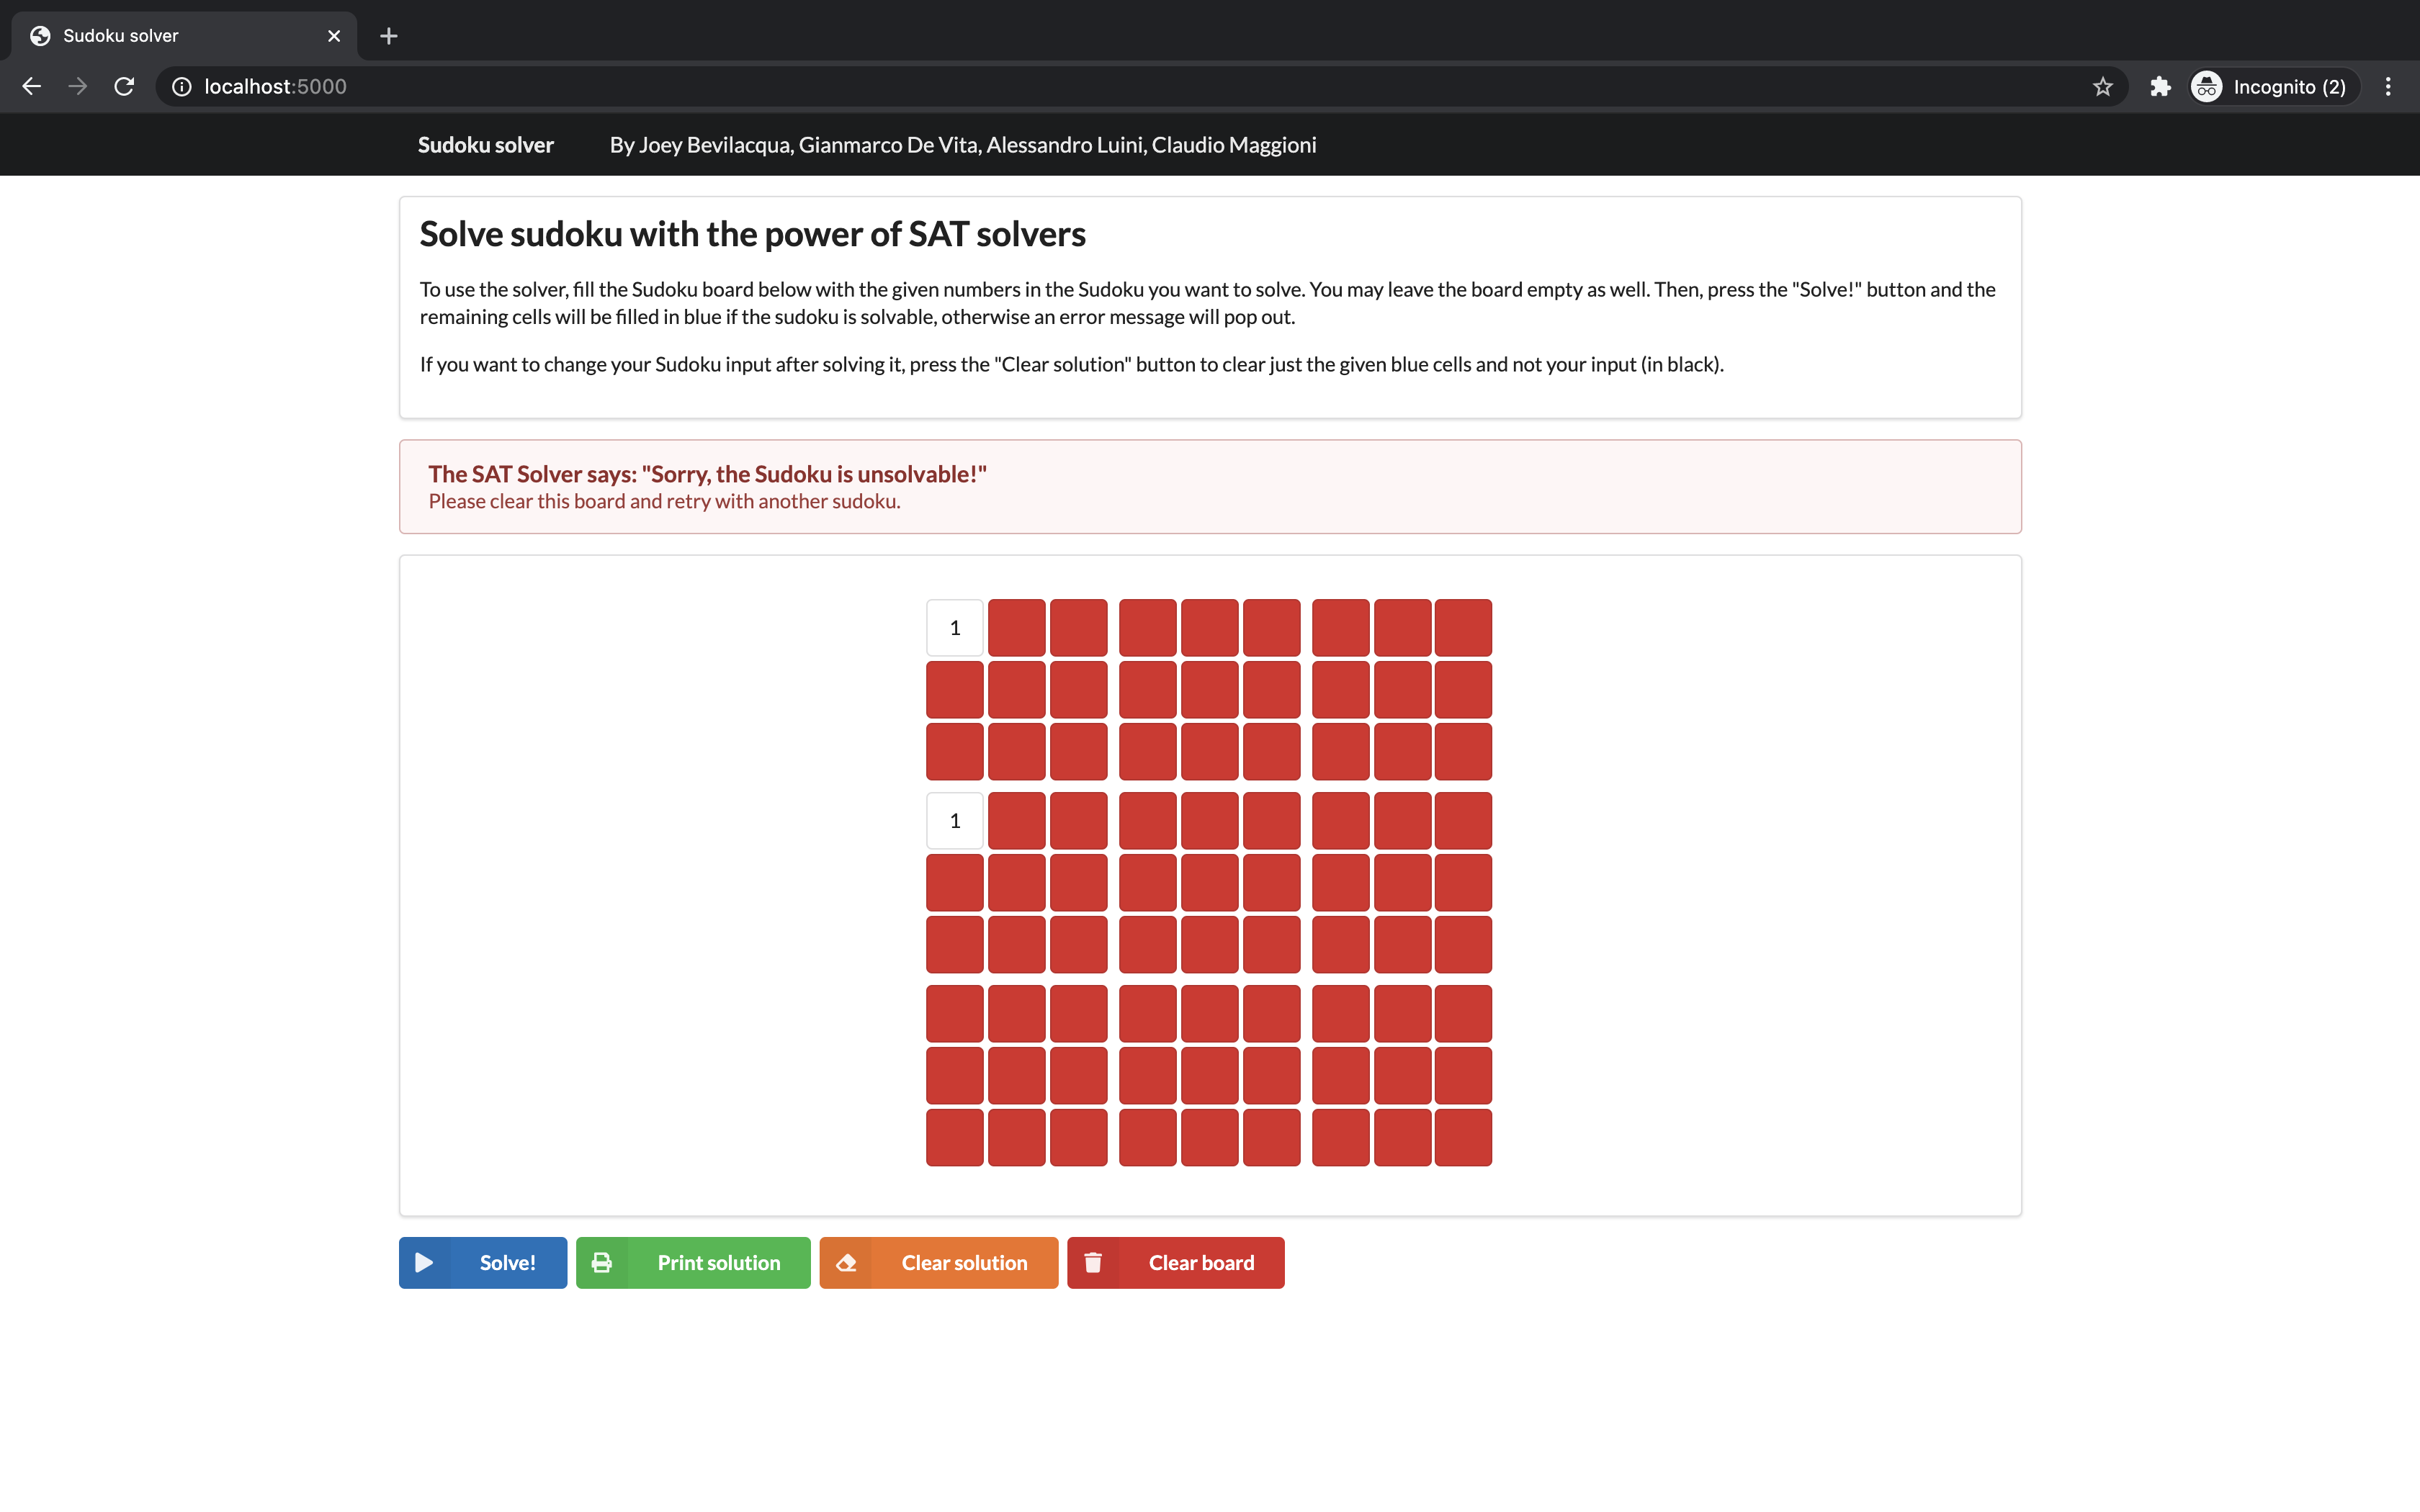
\includegraphics[width=0.8\textwidth]{pics/column_check.png}
\end{figure}

\begin{figure}
\caption{Errors if a number appears multiple times in the same box}
\centering
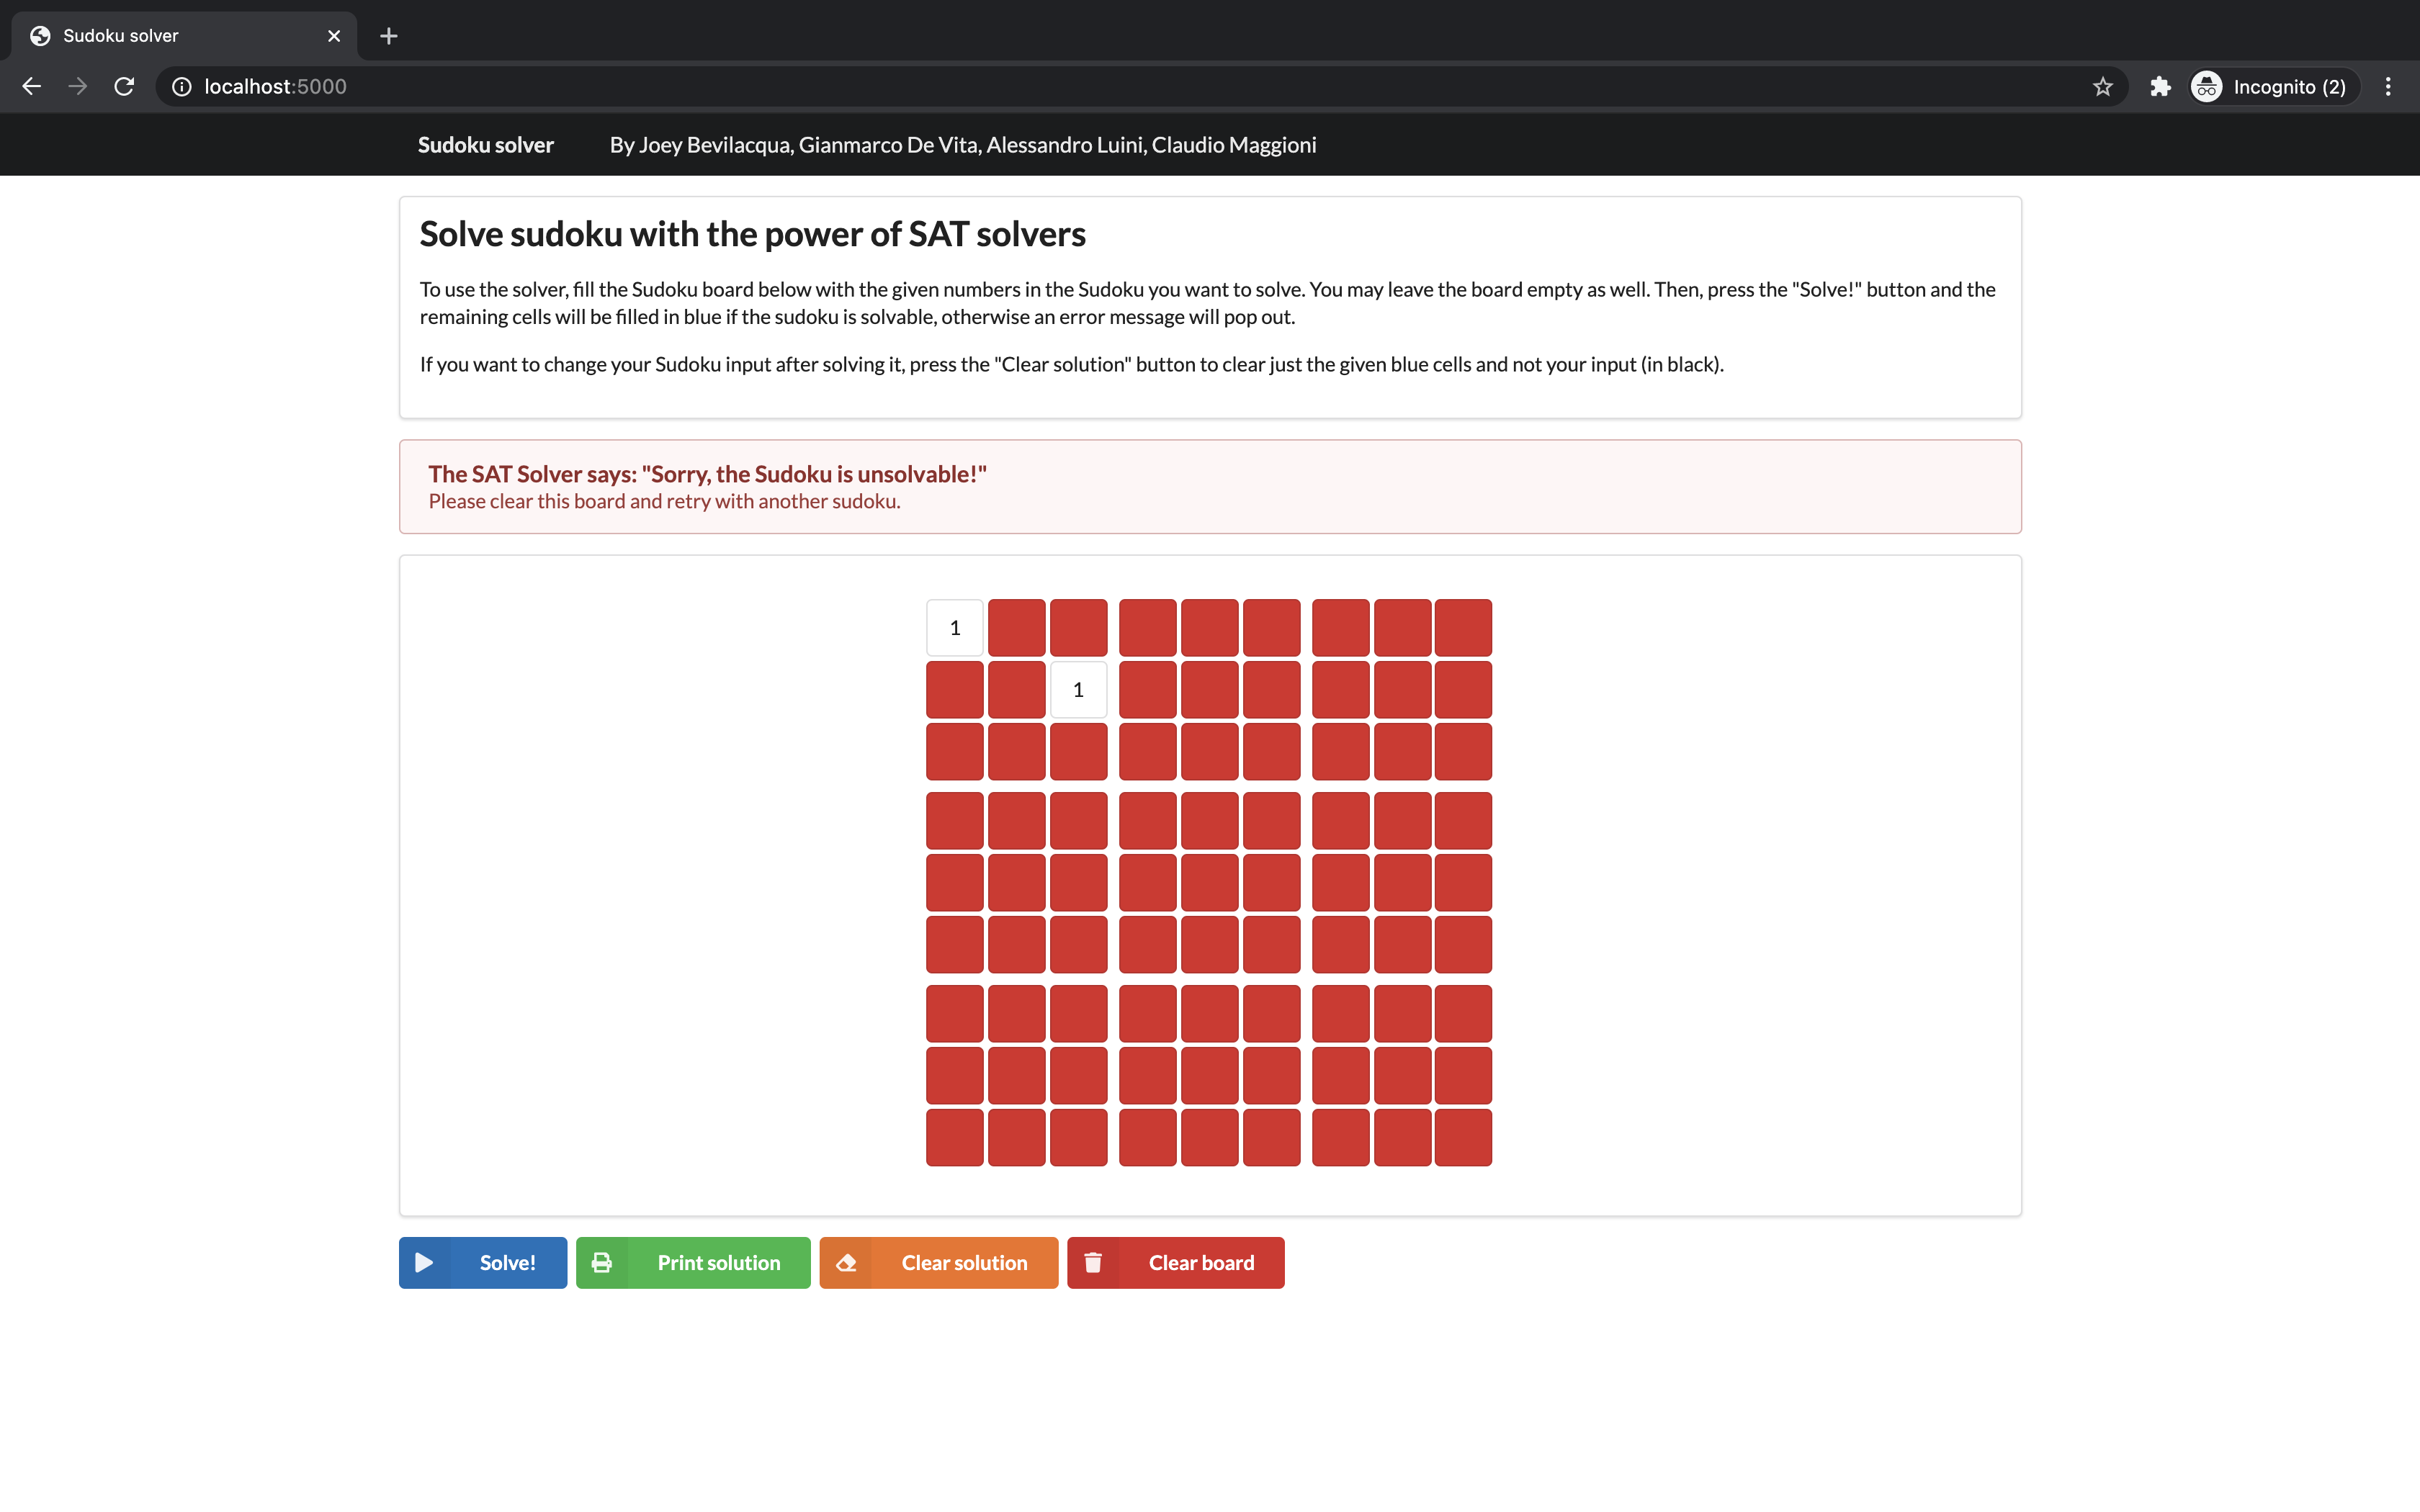
\includegraphics[width=0.8\textwidth]{pics/box_check.png}
\end{figure}

\begin{figure}
\caption{Errors if a number is not in $ \left[ 1, 9 \right] $}
\centering
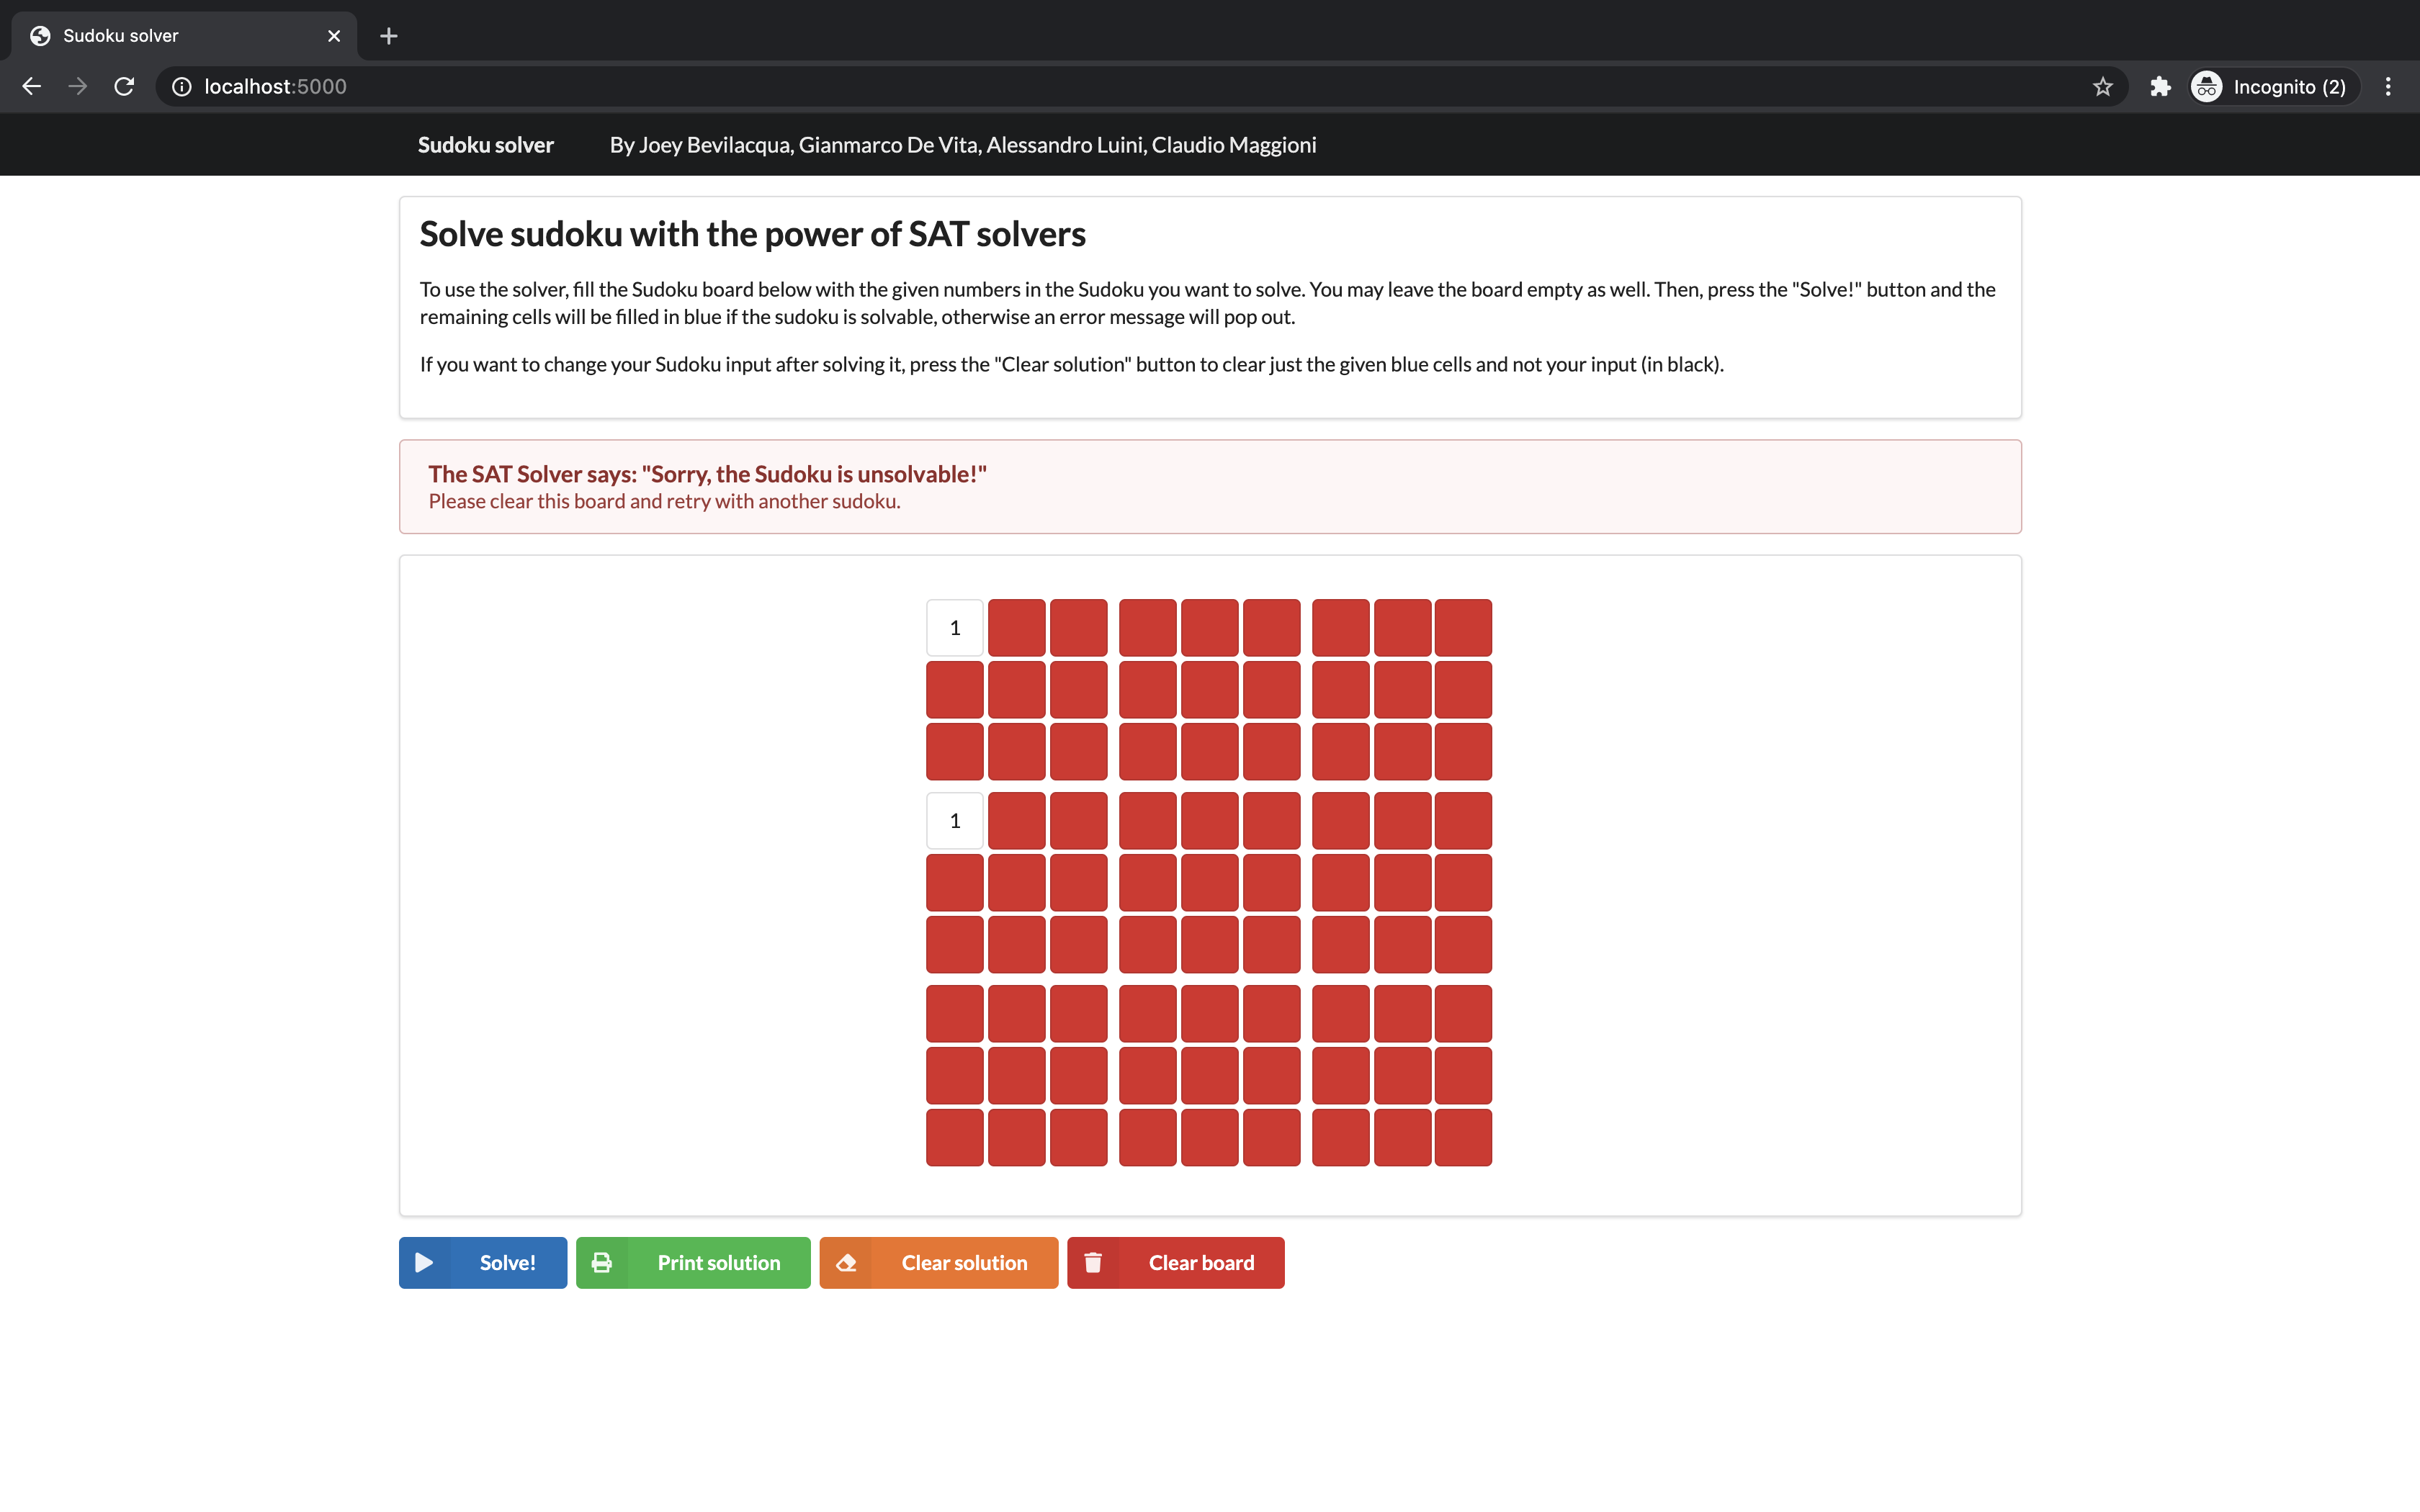
\includegraphics[width=0.8\textwidth]{pics/column_check.png}
\end{figure}

\begin{figure}
\caption{Errors if a number is not in $ \left[ 1, 9 \right] $}
\centering
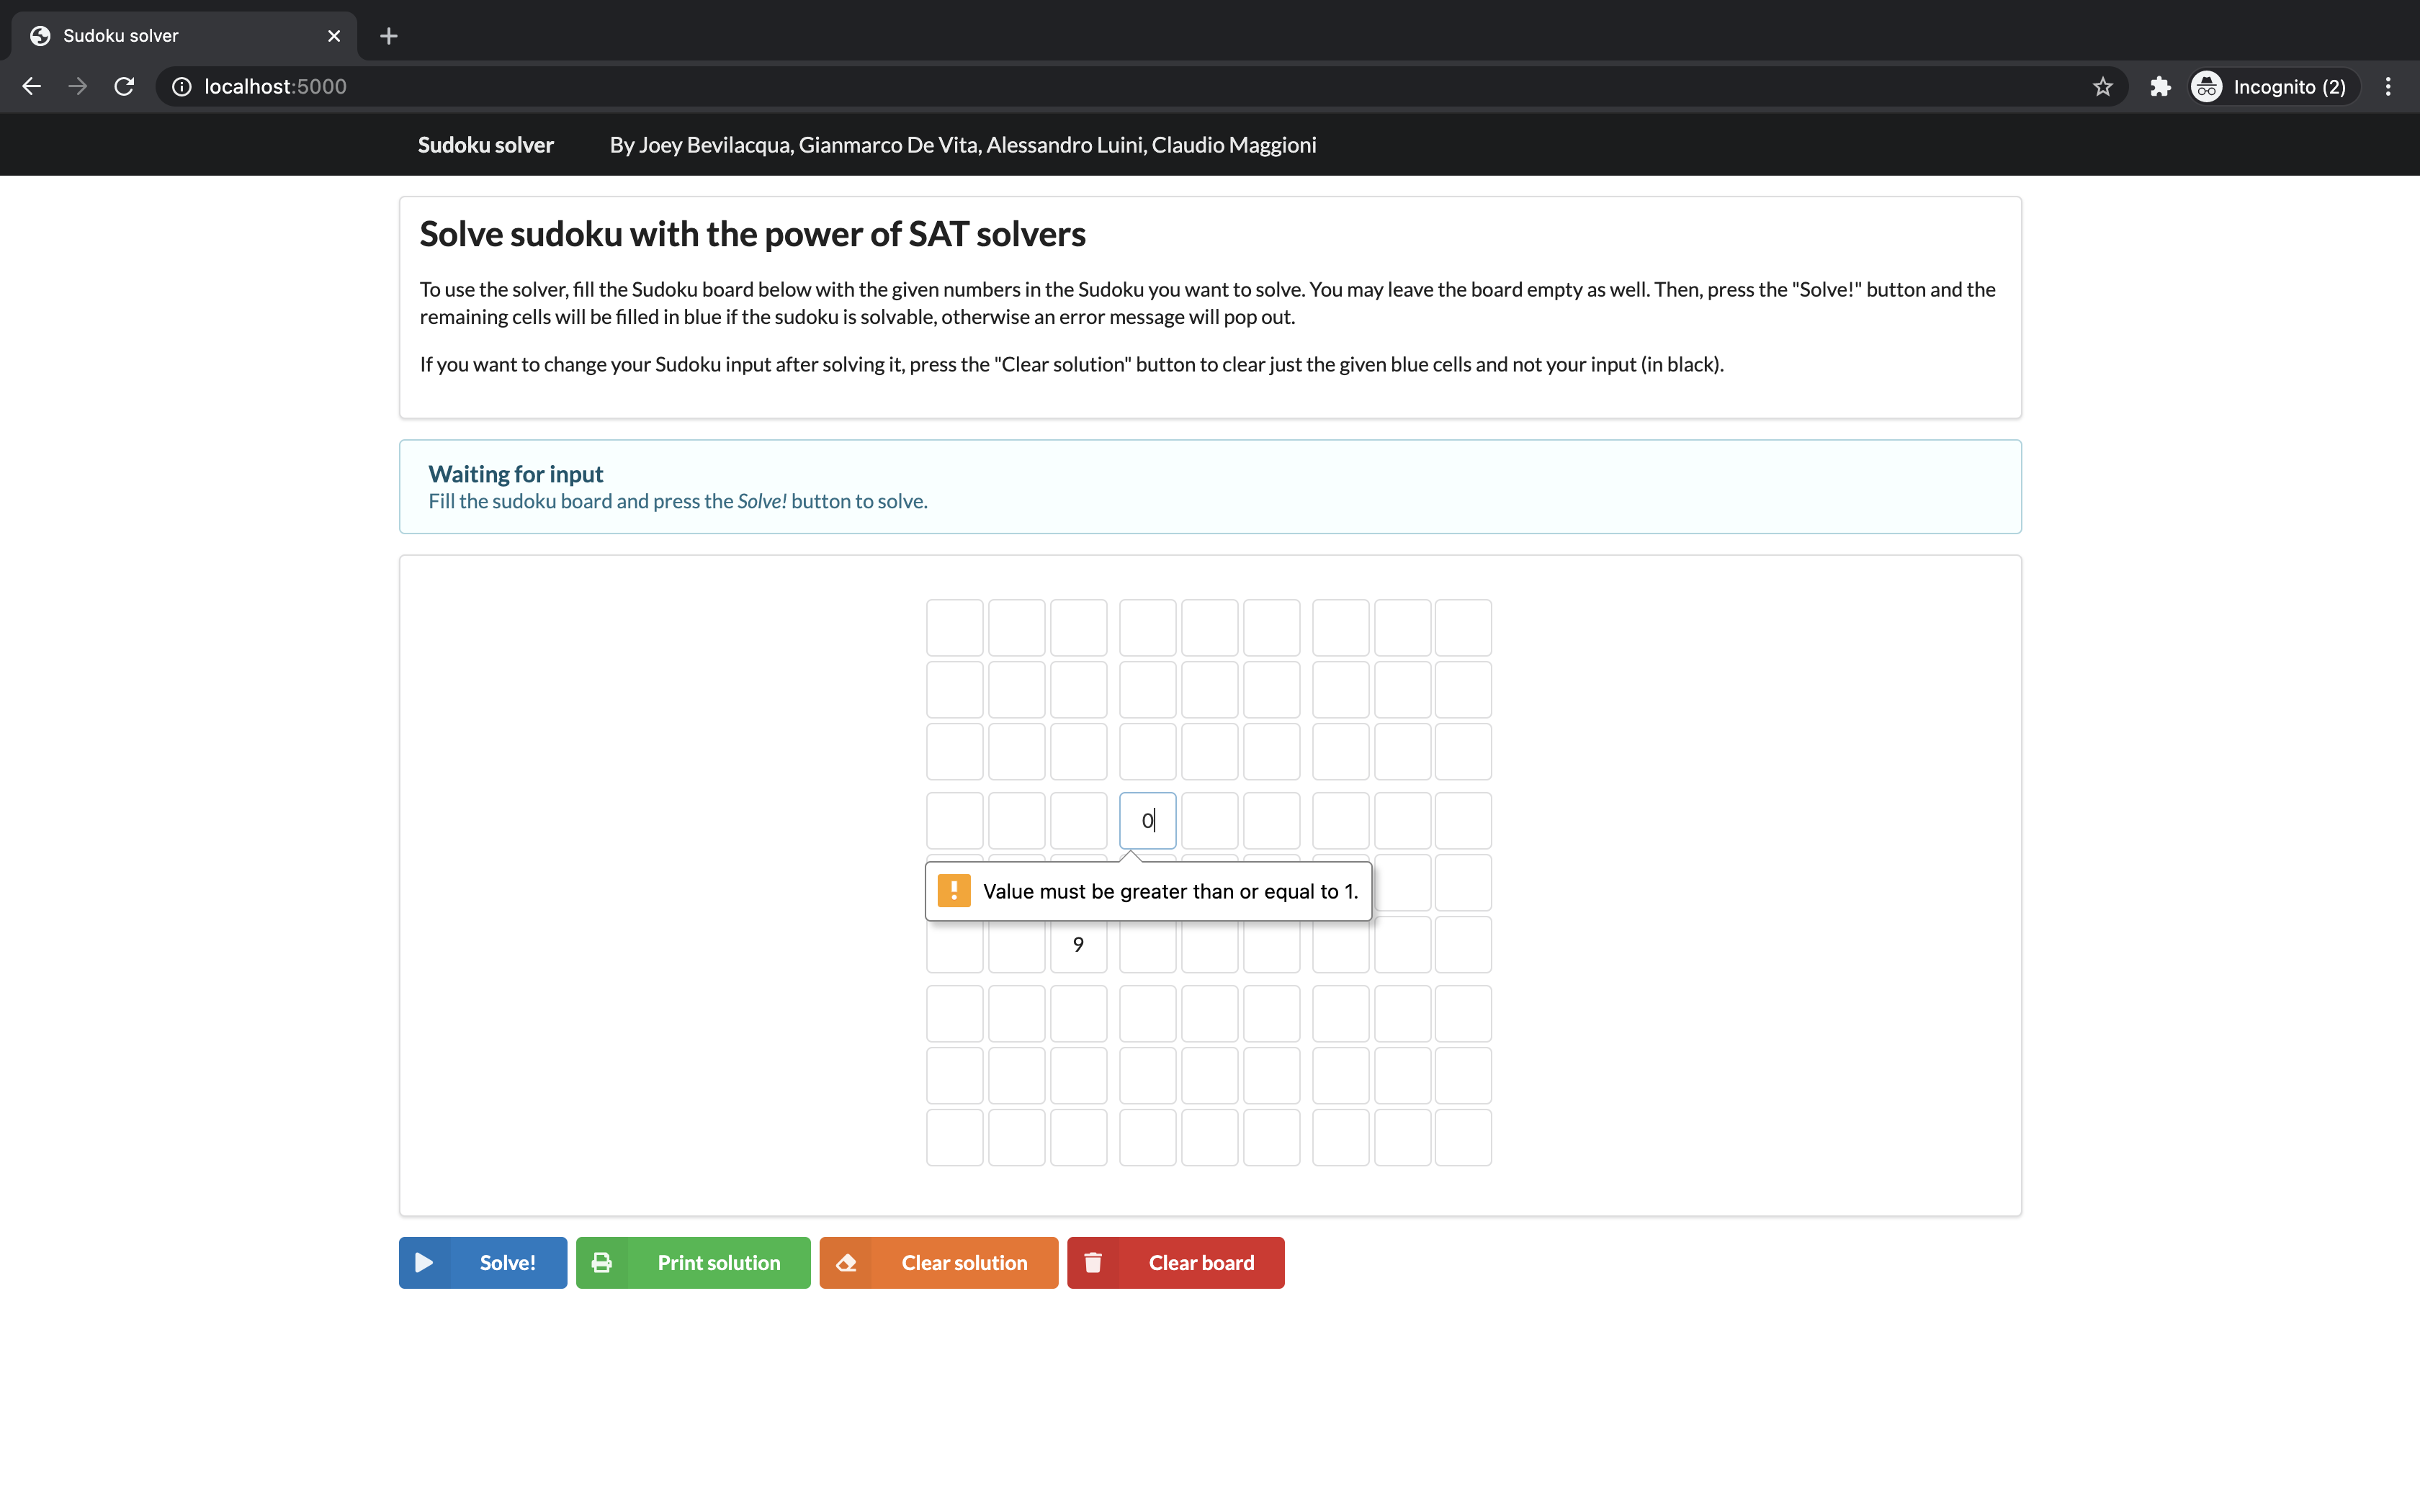
\includegraphics[width=0.8\textwidth]{pics/input_check.png}
\end{figure}

\begin{figure}
\caption{Solve \href{https://www.mirror.co.uk/news/weird-news/worlds-hardest-sudoku-can-you-242294}{the world's hardest sudoku} in seconds}
\centering
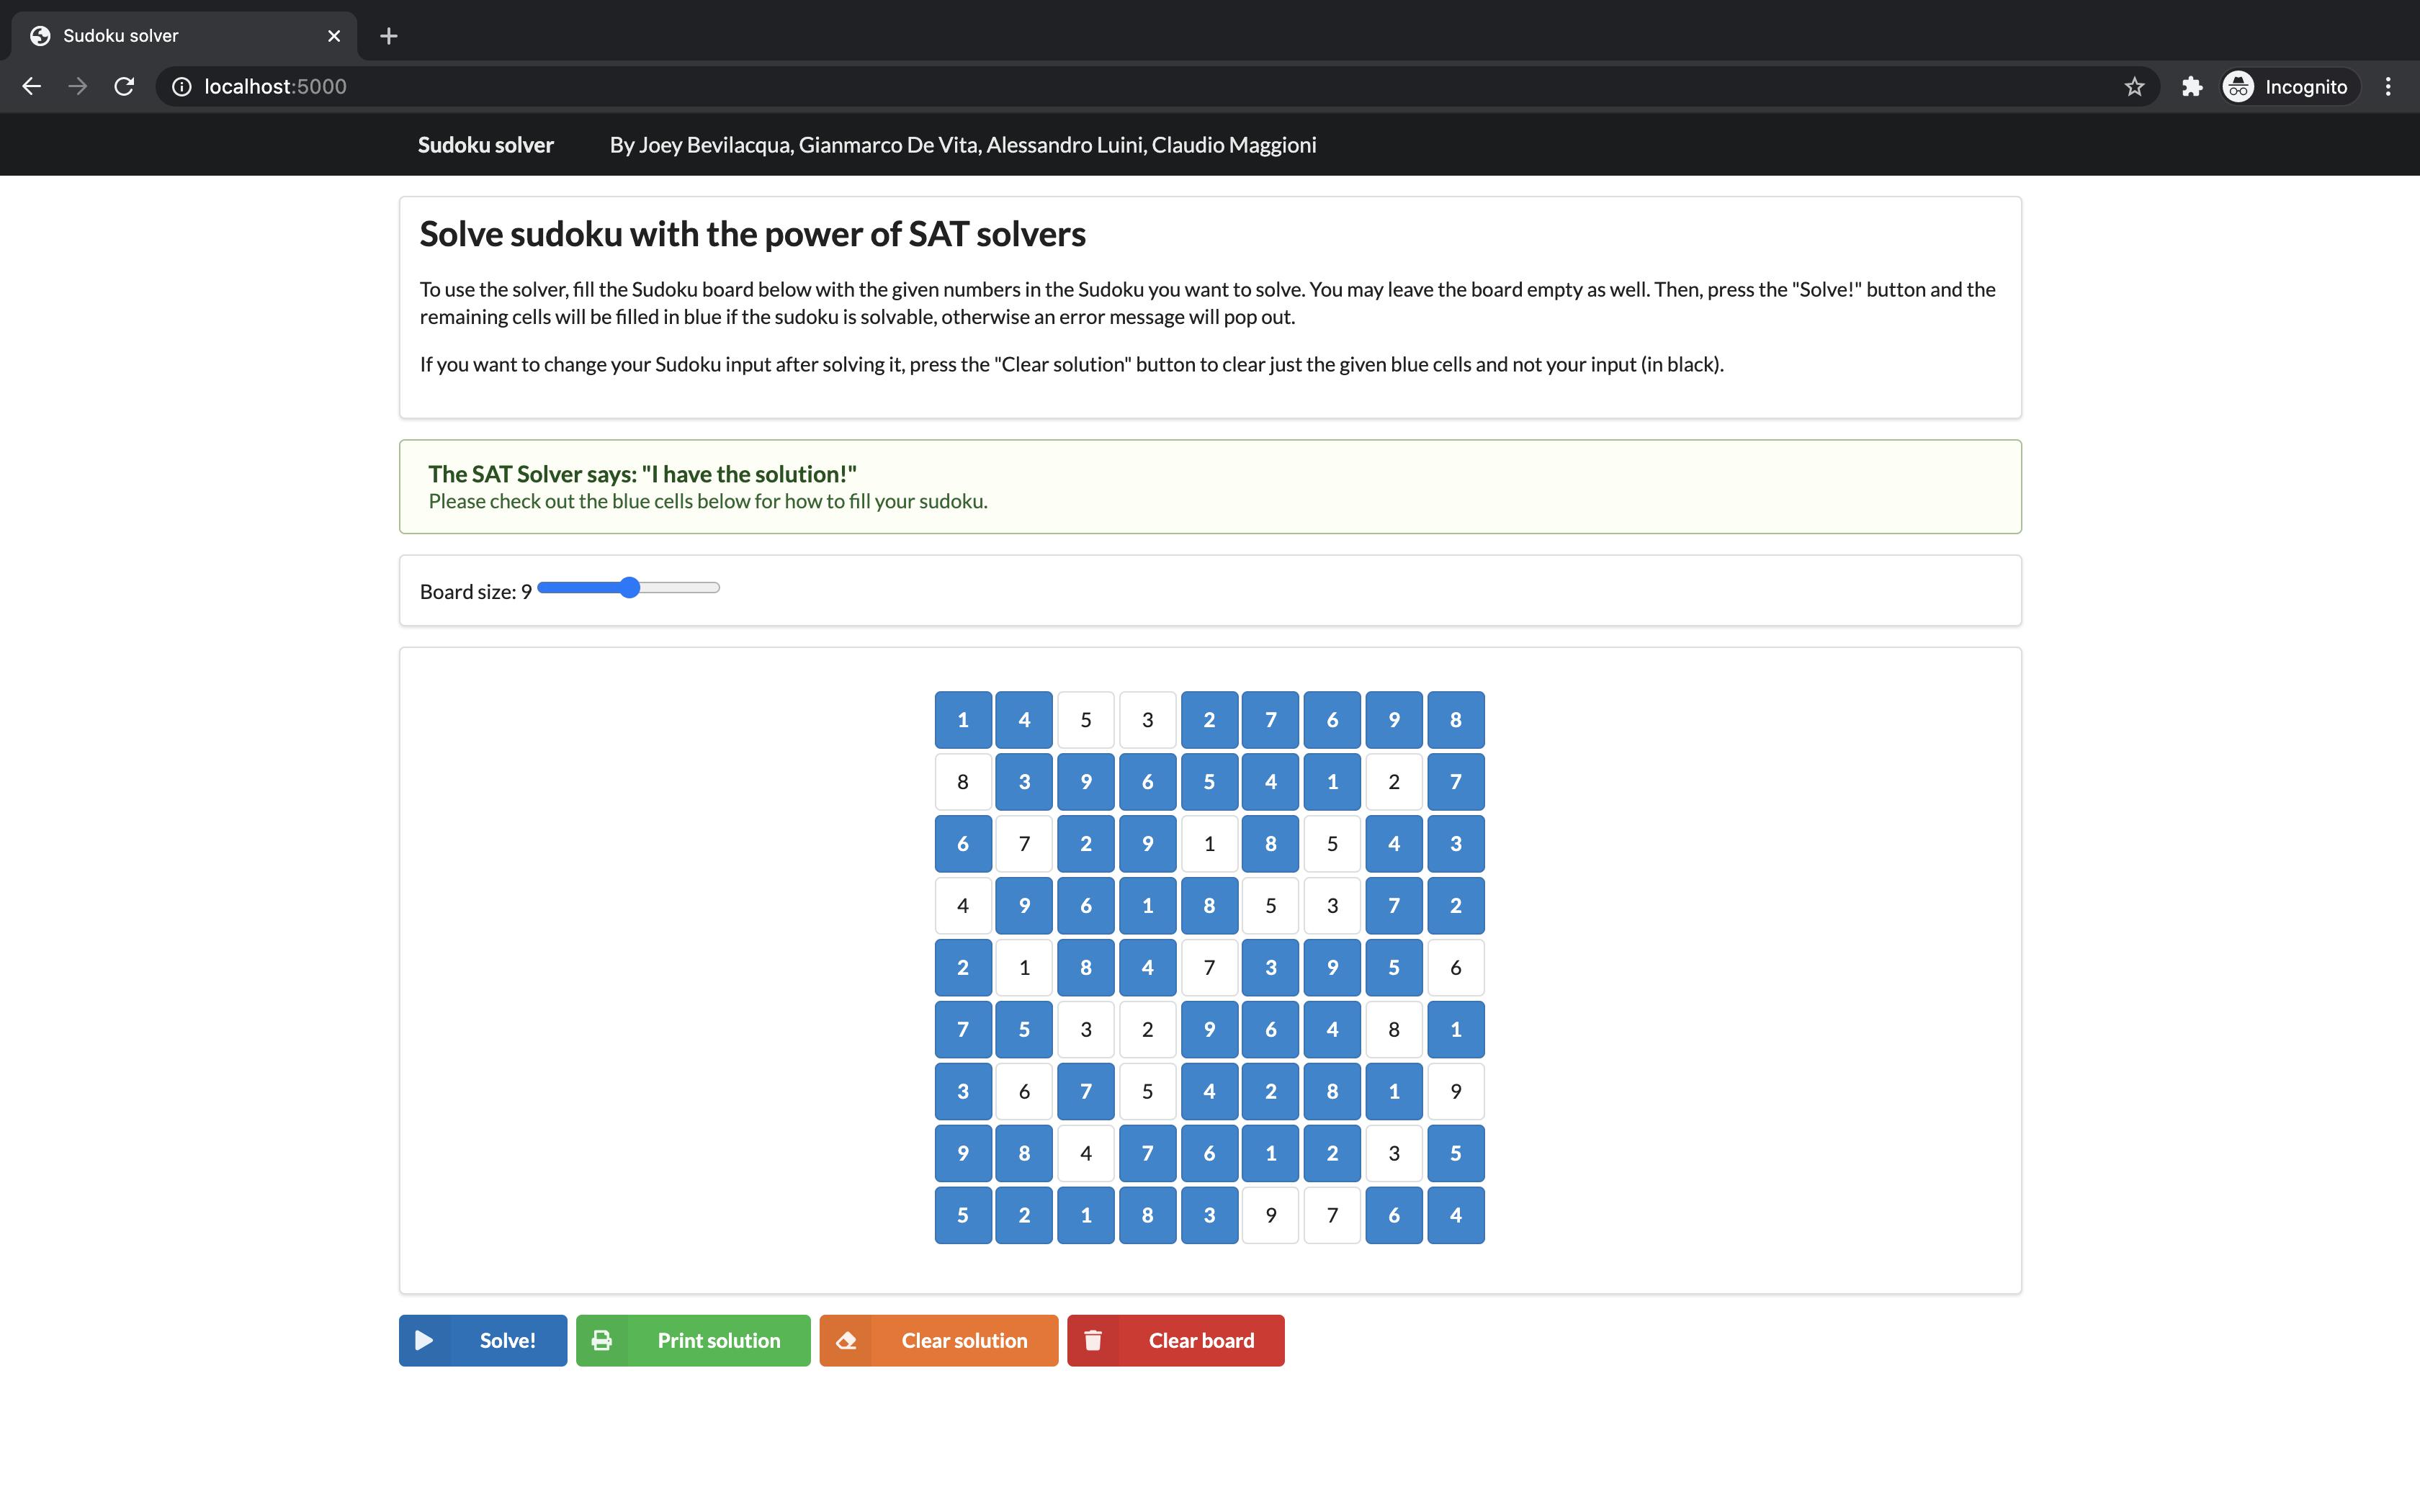
\includegraphics[width=0.8\textwidth]{pics/hardest_sudoku.png}
\end{figure}

%%%%%
\bibliographystyle{abbrv}
\bibliography{references}



\end{document}